%%============
%%  ** Author: Shepherd Qirong
%%  ** Date: 2022-06-05 14:55:53
%%  ** Github: https://github.com/ShepherdQR
%%  ** LastEditors: Shepherd Qirong
%%  ** LastEditTime: 2023-04-09 22:04:52
%%  ** Copyright (c) 2019--20xx Shepherd Qirong. All rights reserved.
%%============


\documentclass[UTF8]{../RepresentationUniverse}
\begin{document}

\title{02-PerformingArts}
\date{Created on 20220605.\\   Last modified on \today.}
\maketitle
\tableofcontents


\chapter{Introduction}

表演艺术

\chapter{音乐}

\section{随同}
\section{室内乐}
\section{教堂音乐}
\section{进行}
    \subsection{合唱指挥}
    \subsection{管弦乐指挥}
    \subsection{管乐团指挥}
\section{早期音乐}
\section{爵士乐研究}
\section{音乐作品}
\section{音乐教育}
\section{音乐史}
\section{音乐学}
\section{历史音乐学}
\section{系统音乐学}
\section{民族音乐学}
\section{音乐理论}
\section{管弦乐研究}
\section{乐器学}
\section{管风琴和历史键盘}
\section{地面}
\section{弦乐、竖琴、沉香木和吉他}
\section{唱歌}
\section{木管乐器、铜管乐器和打击乐器}


\chapter{舞蹈}
\section{编舞}
\section{舞蹈符号}
\section{舞蹈史}

\chapter{电视}


\chapter{剧场}
\section{演戏}
\section{导演}
\section{戏剧艺术}
\section{音乐剧院}
\section{编剧}
\section{木偶戏}
\section{布景}
\section{舞台设计}
\section{腹语术}


\chapter{电影}


\section{纪录片}

\subsection{观看学习}


\subsubsection{BBC: The Genius of Design}
BBC-设计天赋-共5集。

【1】机器之魂

福特Model T,流水线,福特构想的是功能、外观设计,设计师在技术方面重点研究车架。一天生产一大片车,确实是大生意。后来个性化的需求增大,要转变批量的模式。机械工程和外观工艺工程。



【2】民主设计

进入机器时代后,反思人和物的关系。
如椅子需要有几个腿?软布包裹一团空气充当椅子。

Bauhaus的艺术学生,引发新的设计思想。自由的爱恨,先锋的精神,传奇的行为。

Art Nouveau风格:19-20世纪初的设计风格。装饰意味强烈,highly decorated.

圆形钢管影响椅子的设计。椅子难设计,可看出设计师的水平。



\begin{figure}[h]
    \centering
    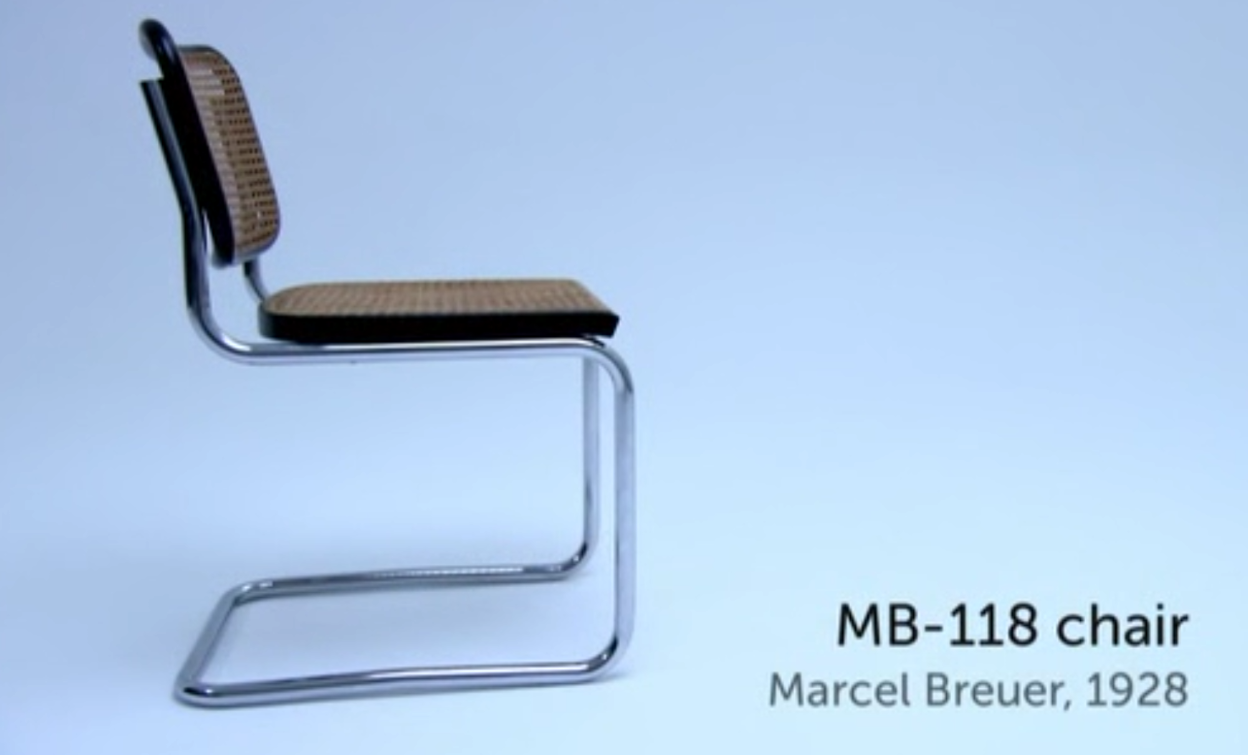
\includegraphics[width=0.5\textwidth]{./src/figures/MB118Chair_2023-04-09_16-42-08.png}
    \caption{[Marcel Breuer:MB118Chair]}
    \label{figure:MB118Chair}
\end{figure}


人机工程,记录工人动作,看他们是怎么提高效率的。记录在厨房中的轨迹路线,设计出布局合理的厨房。缺点是工业化、狭小,没有居家的情调。

\begin{figure}[h]
    \centering
    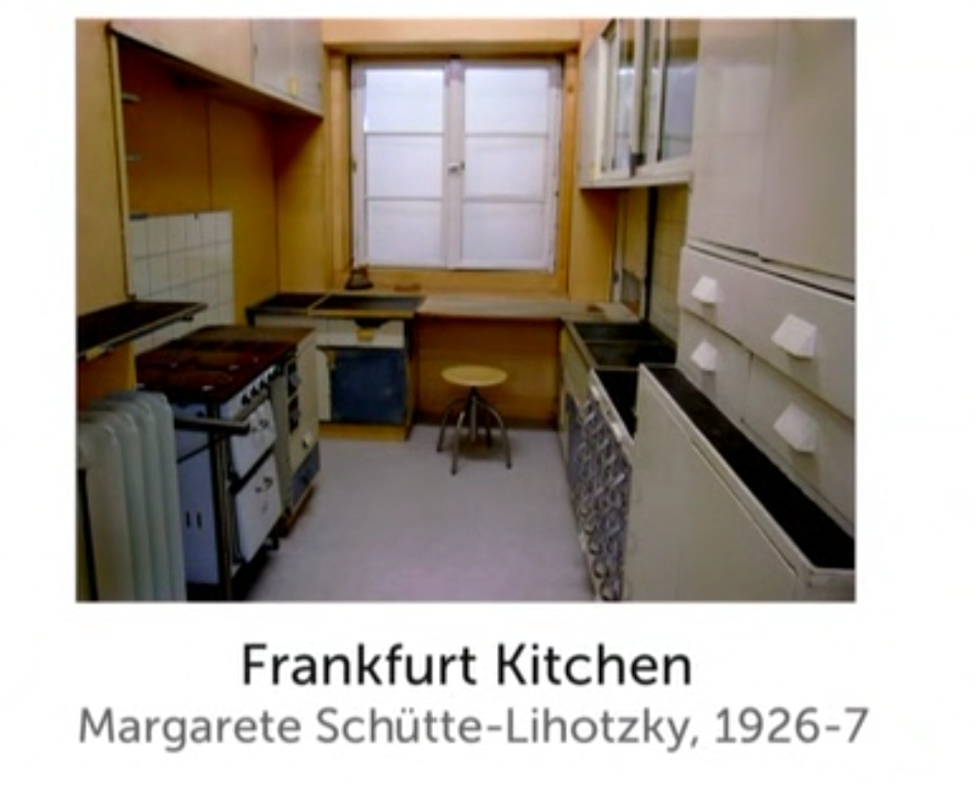
\includegraphics[width=0.5\textwidth]{./src/figures/Frankfurt Kitchen_2023-04-09_16-48-37.png}
    \caption{[Margarete:Frankfurt Kitchen]}
    \label{figure:Frankfurt Kitchen}
\end{figure}

\begin{figure}[h]
    \centering
    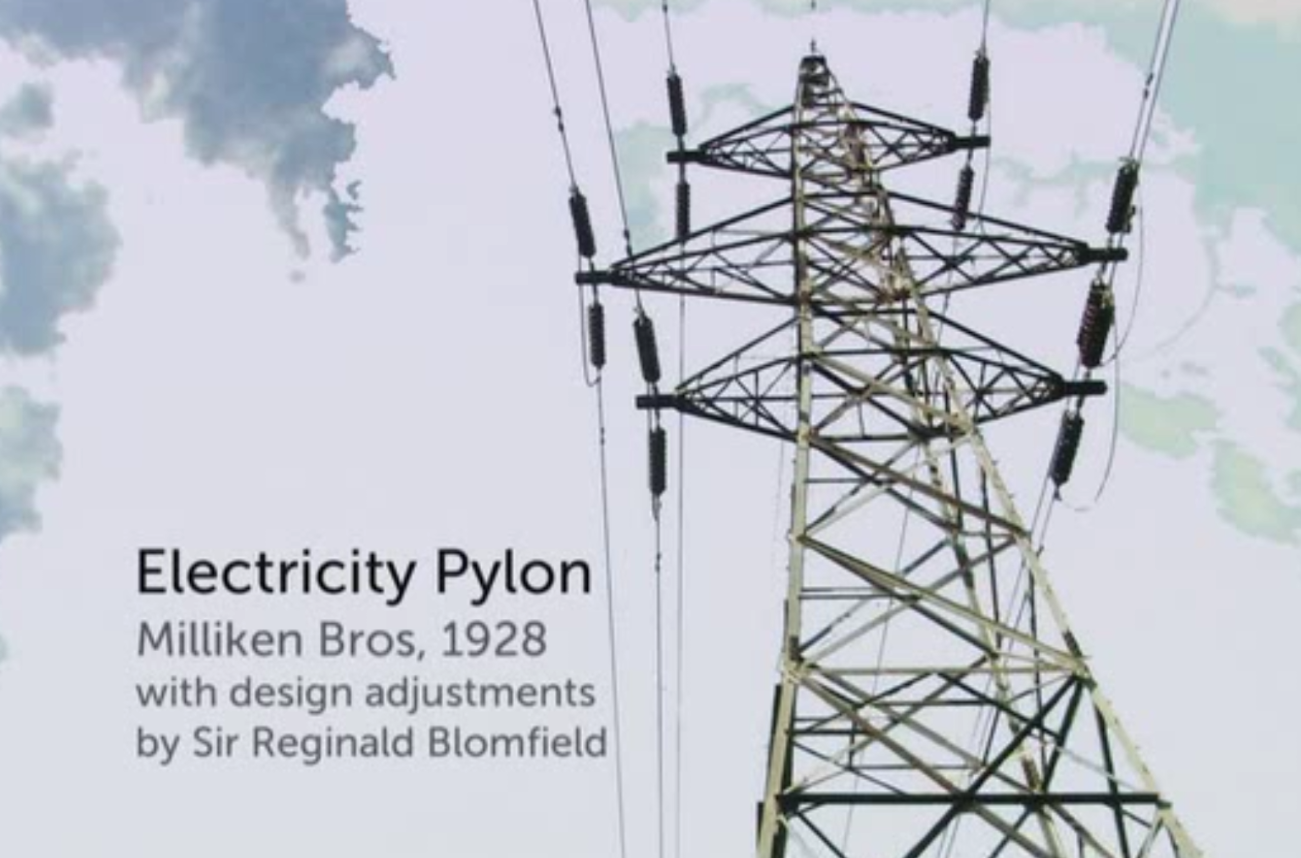
\includegraphics[width=0.5\textwidth]{./src/figures/Electricity Pylon_2023-04-09_19-18-02.png}
    \caption{[Milliken Bros:Electricity Pylon]}
    \label{figure:Electricity Pylon}
\end{figure}



\begin{figure}[h]
    \centering
    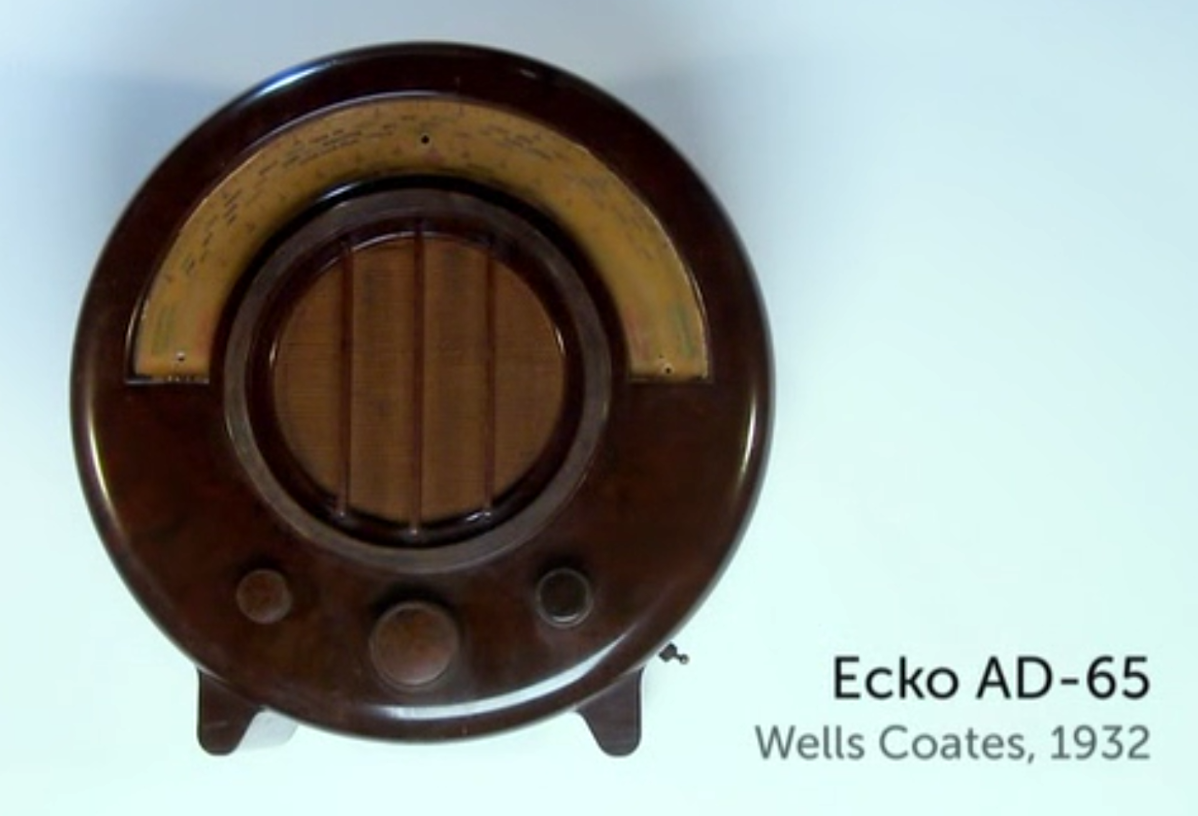
\includegraphics[width=0.5\textwidth]{./src/figures/Ecko AD65_2023-04-09_19-20-05.png}
    \caption{[Wells Coates:Ecko AD65]}
    \label{figure:Ecko AD65}
\end{figure}


\begin{figure}[h]
    \centering
    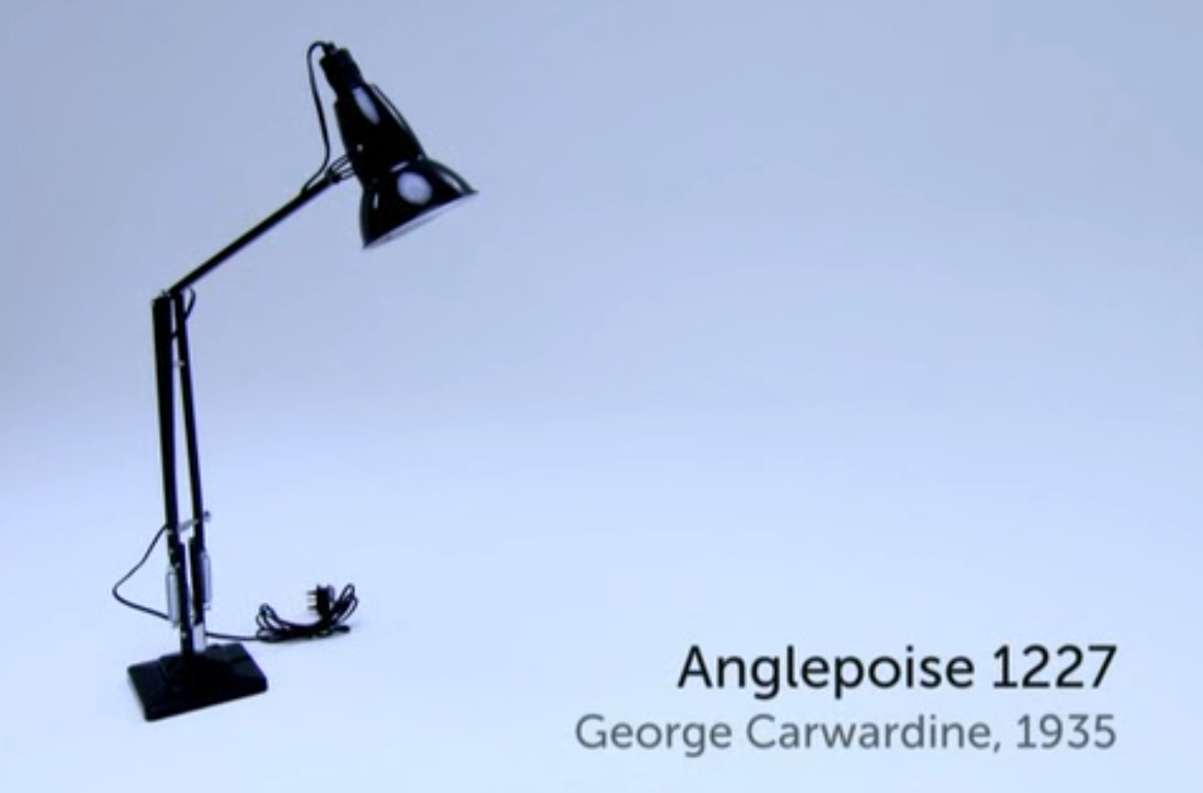
\includegraphics[width=0.5\textwidth]{./src/figures/Anglepoise1227_2023-04-09_19-21-53.png}
    \caption{[George Carwardine:Anglepoise1227]}
    \label{figure:Anglepoise1227}
\end{figure}


Le Corbusier 抱怨曼哈顿的大楼太密集且too small,虽然他只是设计过一些小型别墅。

资本主义、用户至上、追求个性,决定美国的未来走向。市场是美国的主宰。

most advanced yet acceptable. 



\begin{figure}[h]
    \centering
    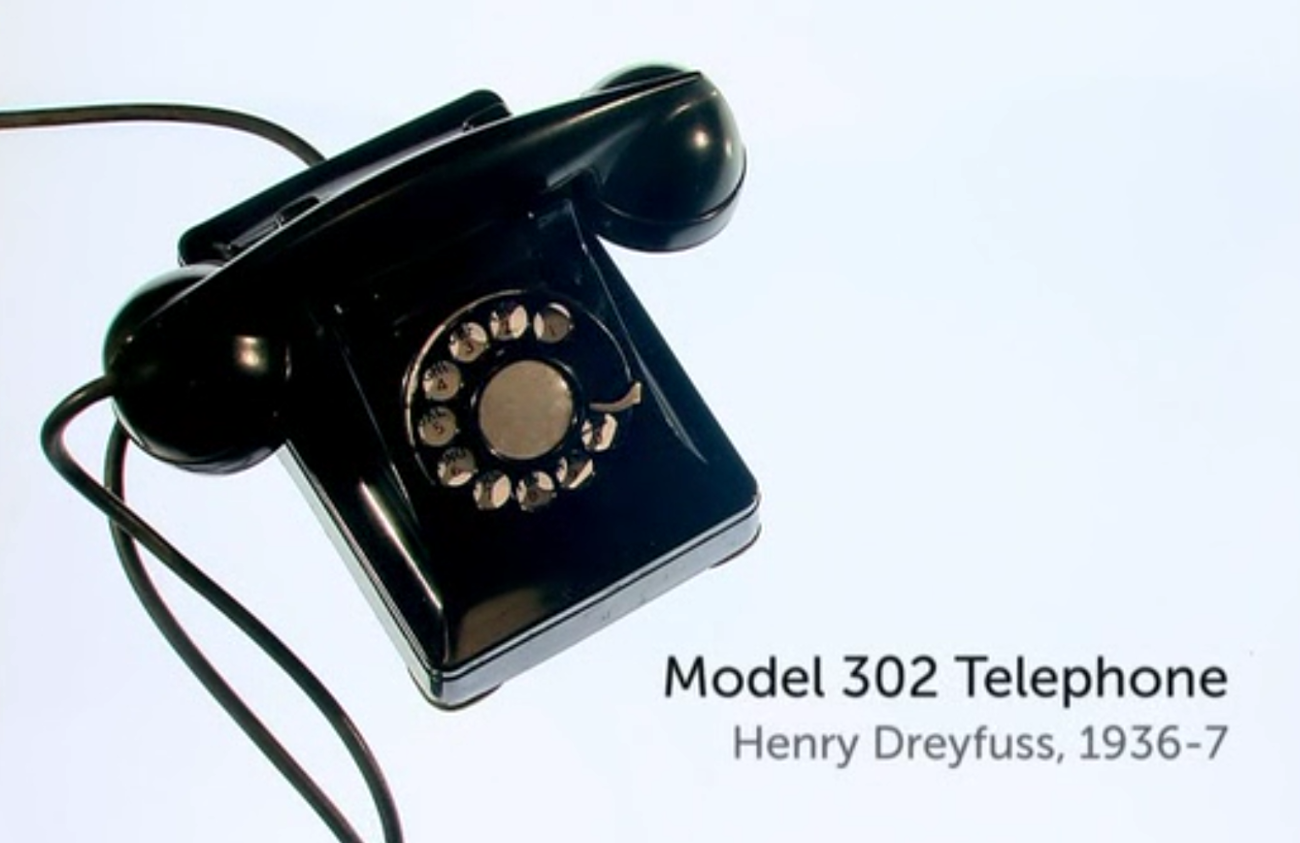
\includegraphics[width=0.5\textwidth]{./src/figures/Model302Telephone_2023-04-09_19-31-13.png}
    \caption{[Henry Dreyfuss:Model302Telephone]}
    \label{figure:Model302Telephone}
\end{figure}


\begin{figure}[h]
    \centering
    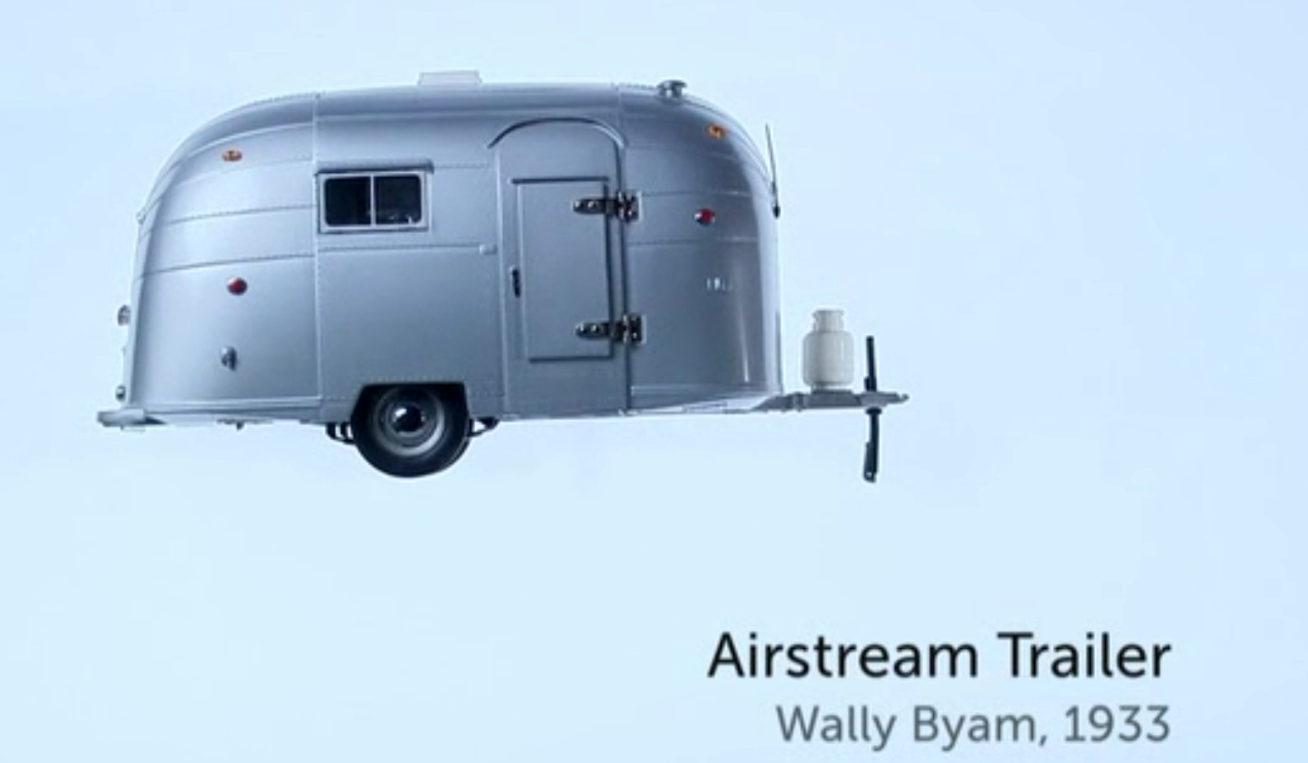
\includegraphics[width=0.5\textwidth]{./src/figures/Airstream Trailer_2023-04-09_19-34-02.png}
    \caption{[Wally Byam:Airstream Trailer]}
    \label{figure:Airstream Trailer}
\end{figure}


【3】战争时代。The ability to do things in great number.

德国。


\begin{figure}[h]
    \centering
    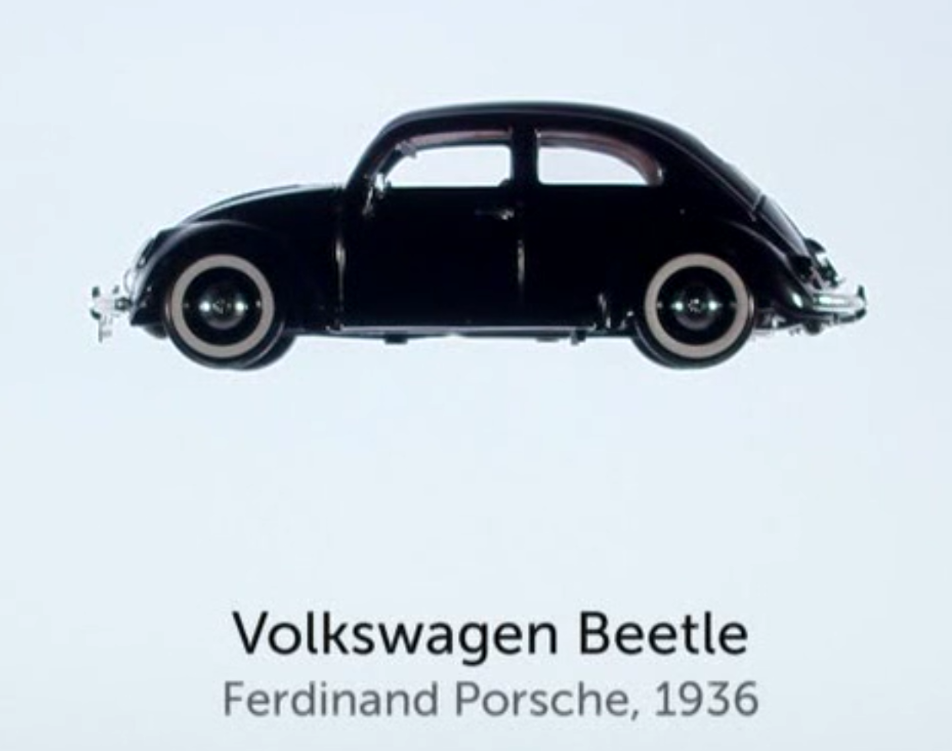
\includegraphics[width=0.5\textwidth]{./src/figures/Volkswagen Beetle_2023-04-09_19-47-01.png}
    \caption{[Ferdinand Porsche:Volkswagen Beetle]}
    \label{figure:Volkswagen Beetle}
\end{figure}

\begin{figure}[h]
    \centering
    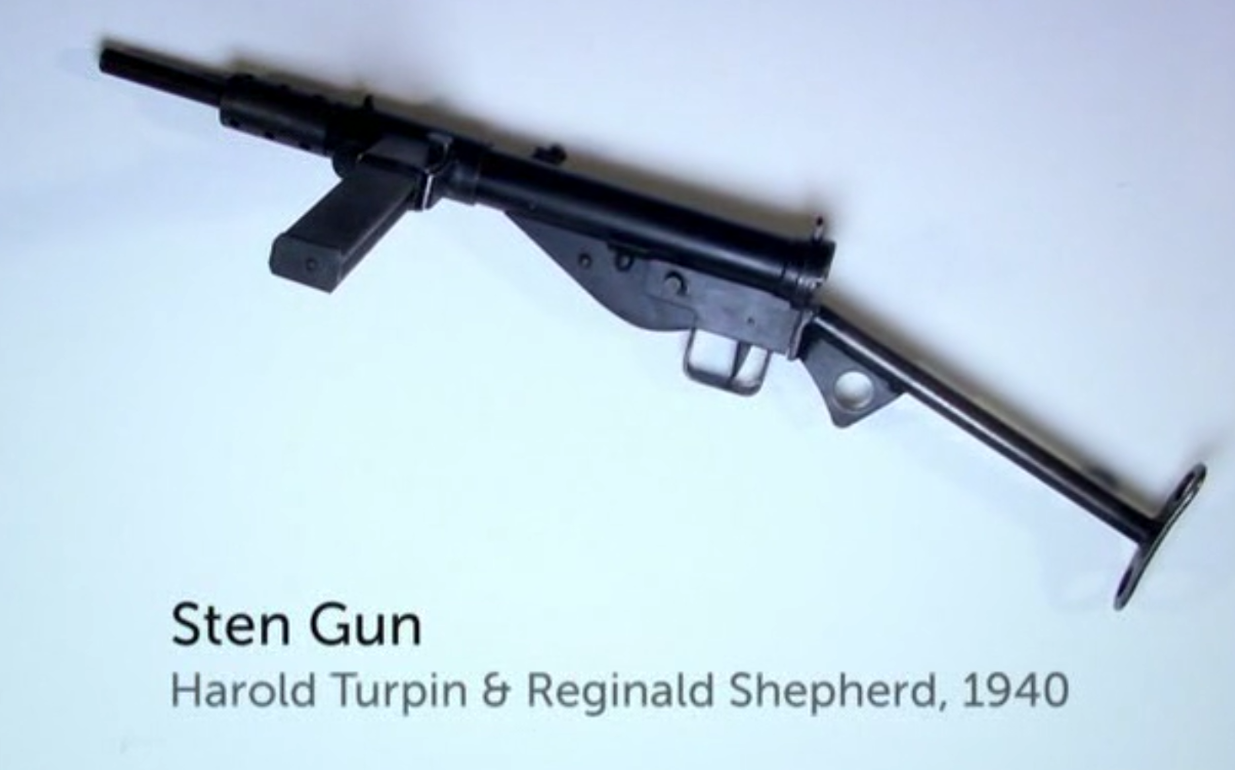
\includegraphics[width=0.5\textwidth]{./src/figures/Sten Gun_2023-04-09_19-51-44.png}
    \caption{[Harold Turpin, Reginald Shepherd:Sten Gun]}
    \label{figure:Sten Gun}
\end{figure}



当时金属紧缺。木质战机。一整片机翼。
\begin{figure}[h]
    \centering
    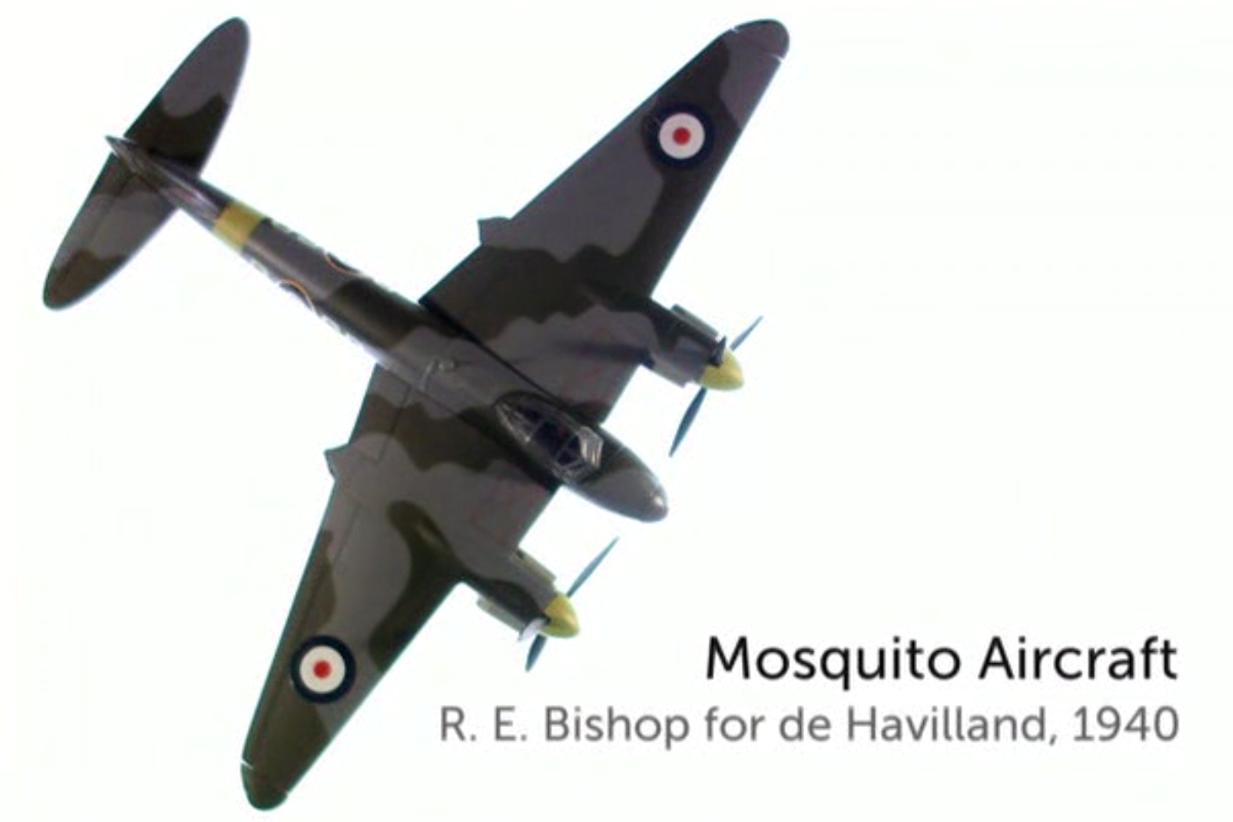
\includegraphics[width=0.5\textwidth]{./src/figures/Mosquito Aircraft_2023-04-09_20-09-31.png}
    \caption{[R.E. Bishop for de Havilland:Mosquito Aircraft]}
    \label{figure:Mosquito Aircraft}
\end{figure}


\begin{figure}[h]
    \centering
    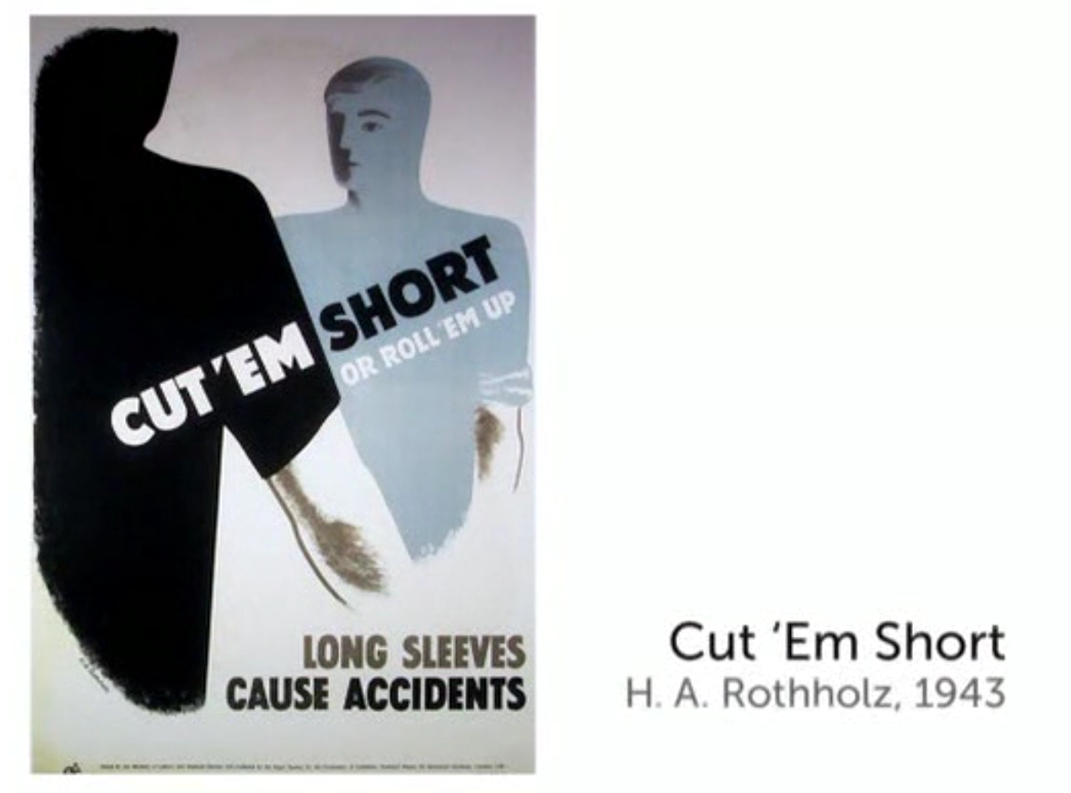
\includegraphics[width=0.5\textwidth]{./src/figures/Cut 'Em Short_2023-04-09_20-13-40.png}
    \caption{[H.A.Rothholz:Cut 'Em Short]}
    \label{figure:Cut 'Em Short}
\end{figure}


\begin{figure}[h]
    \centering
    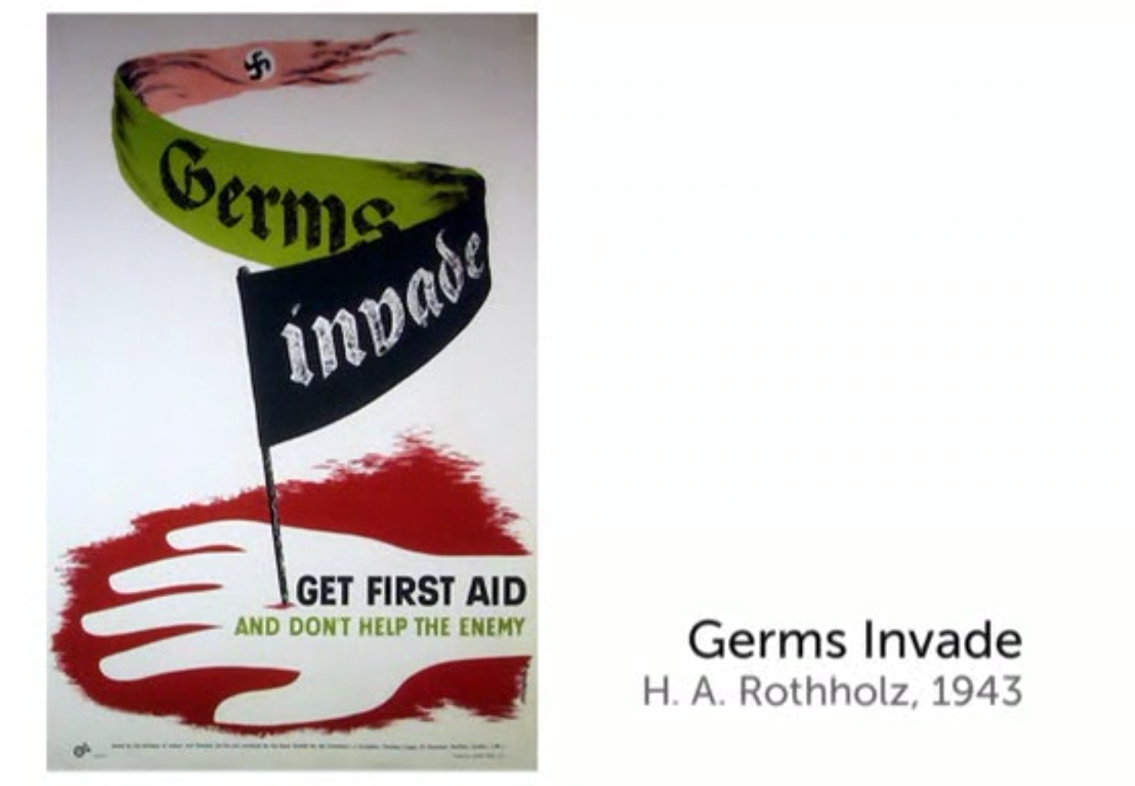
\includegraphics[width=0.5\textwidth]{./src/figures/Germs Invade_2023-04-09_20-15-26.png}
    \caption{[H.A.Rothholz:Germs Invade]}
    \label{figure:Germs Invade}
\end{figure}


Tiger tank 设计精巧,太耗费资源。虎式I坦克早1300辆,俄罗斯的T34可以造60000辆。
\begin{figure}[h]
    \centering
    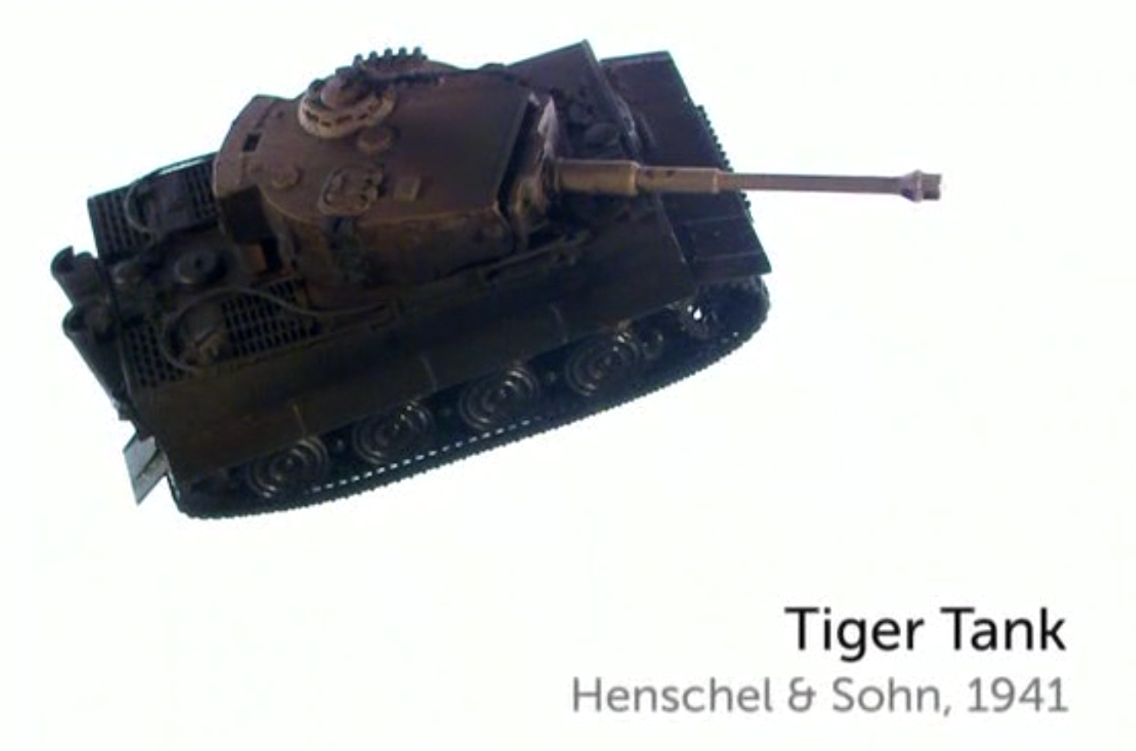
\includegraphics[width=0.5\textwidth]{./src/figures/Tiger Tank_2023-04-09_20-17-37.png}
    \caption{[Henschel and Sohn:Tiger Tank]}
    \label{figure:Tiger Tank}
\end{figure}

\begin{figure}[h]
    \centering
    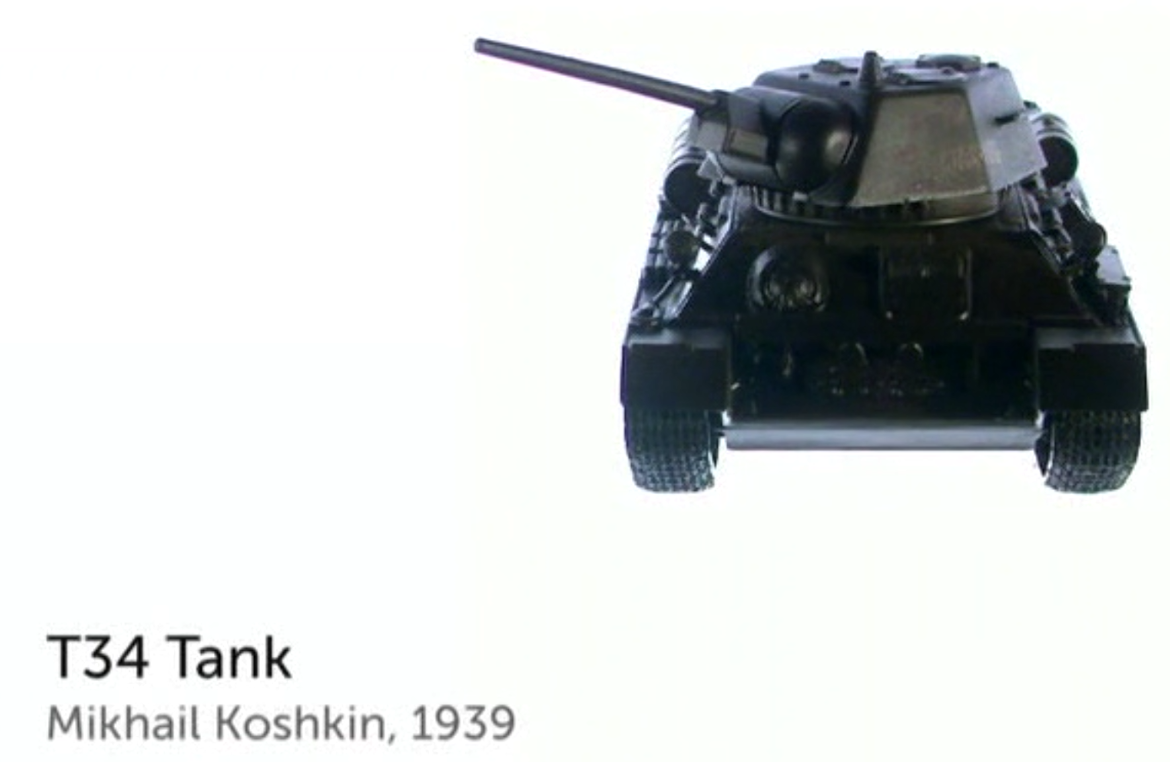
\includegraphics[width=0.5\textwidth]{./src/figures/T34 Tank_2023-04-09_20-22-47.png}
    \caption{[Mikhail Koshkin:T34 Tank]}
    \label{figure:T34 Tank}
\end{figure}

美国,1h生产一架成品飞机。


\begin{figure}[h]
    \centering
    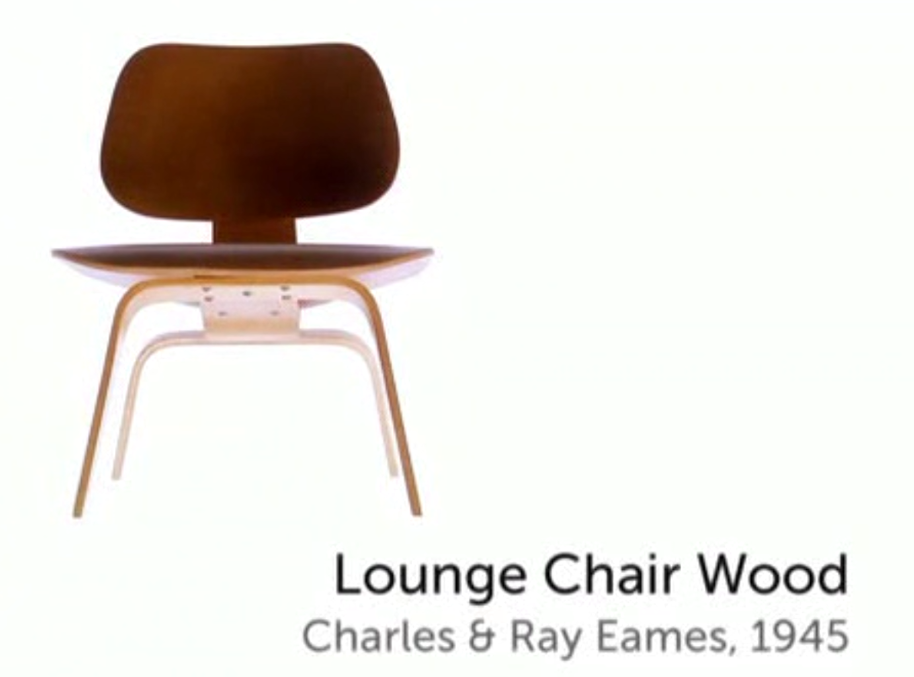
\includegraphics[width=0.5\textwidth]{./src/figures/Lounge Chair Wood_2023-04-09_20-27-26.png}
    \caption{[Charles and Ray Eames:Lounge Chair Wood]}
    \label{figure:Lounge Chair Wood}
\end{figure}
In 1000, time magazine named this chair, the chair of the century.


\begin{figure}[h]
    \centering
    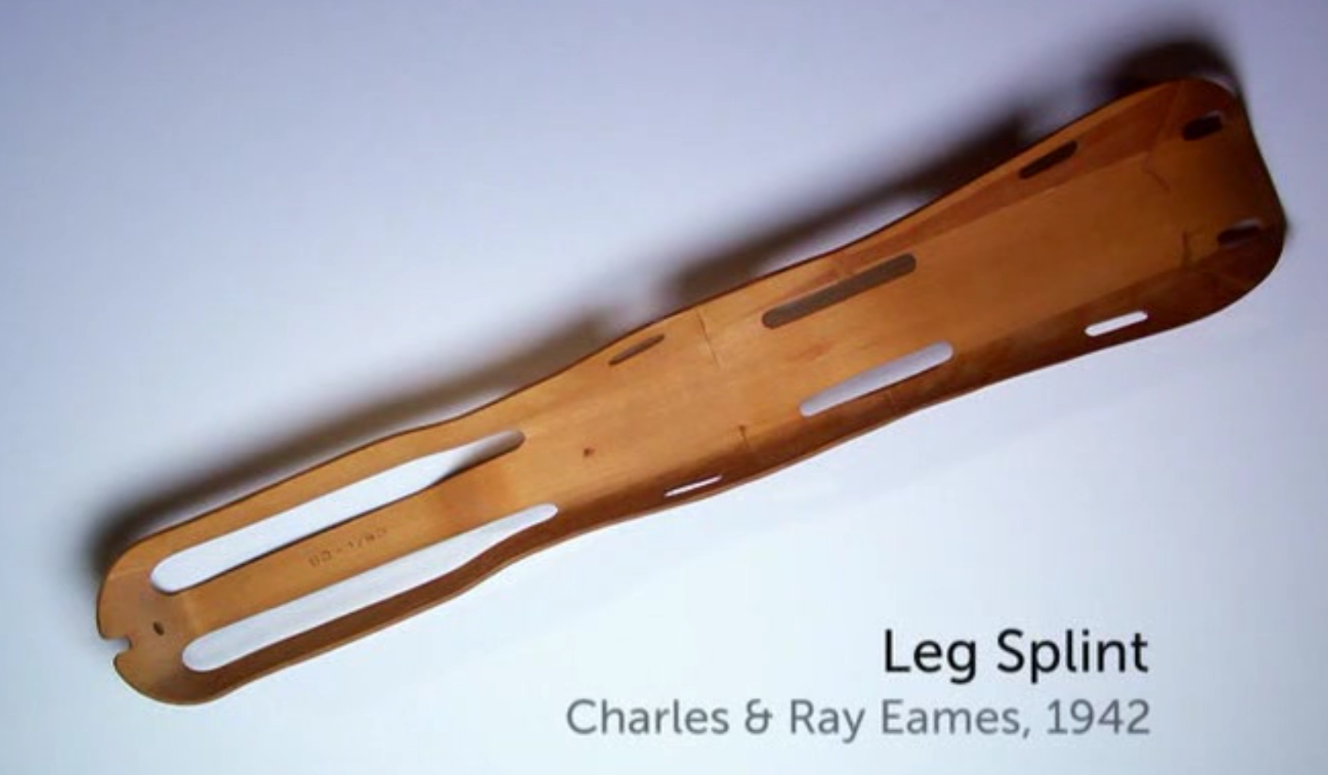
\includegraphics[width=0.5\textwidth]{./src/figures/Leg Splint_2023-04-09_20-30-14.png}
    \caption{[Charles and Ray Eames:Leg Splint]}
    \label{figure:Leg Splint}
\end{figure}



【4】材料革命

二战后美国最受益。
\begin{figure}[h]
    \centering
    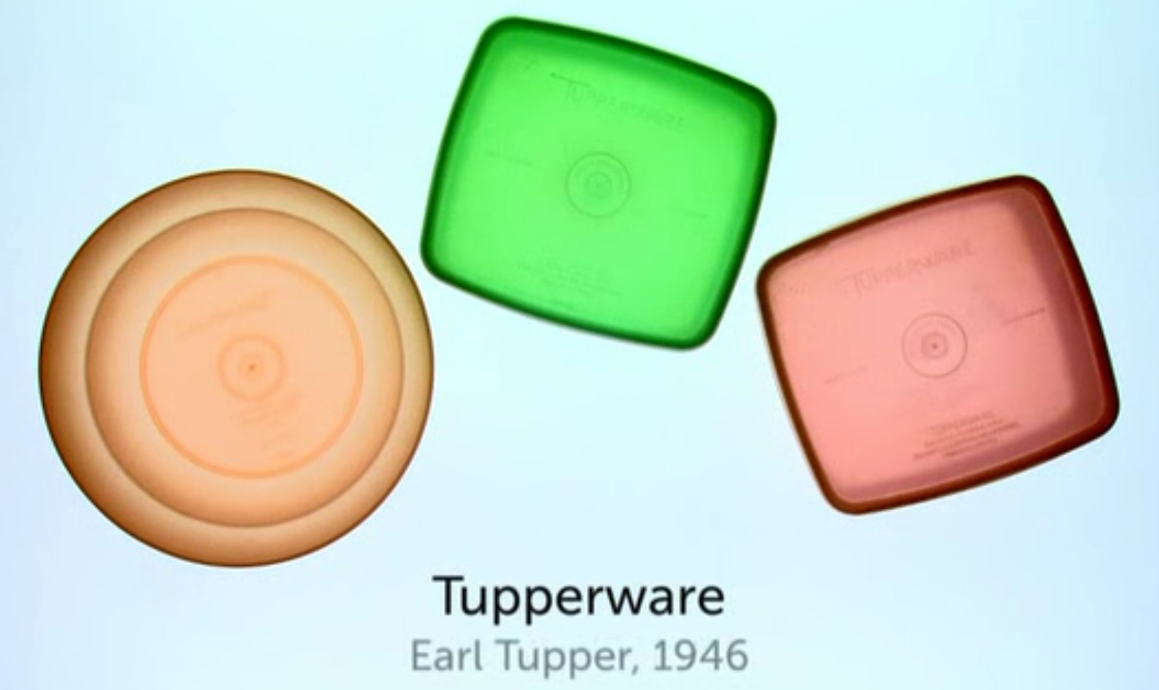
\includegraphics[width=0.5\textwidth]{./src/figures/Tupperware_2023-04-09_20-37-50.png}
    \caption{[Earl Tupper:Tupperware]}
    \label{figure:Tupperware}
\end{figure}



\begin{figure}[h]
    \centering
    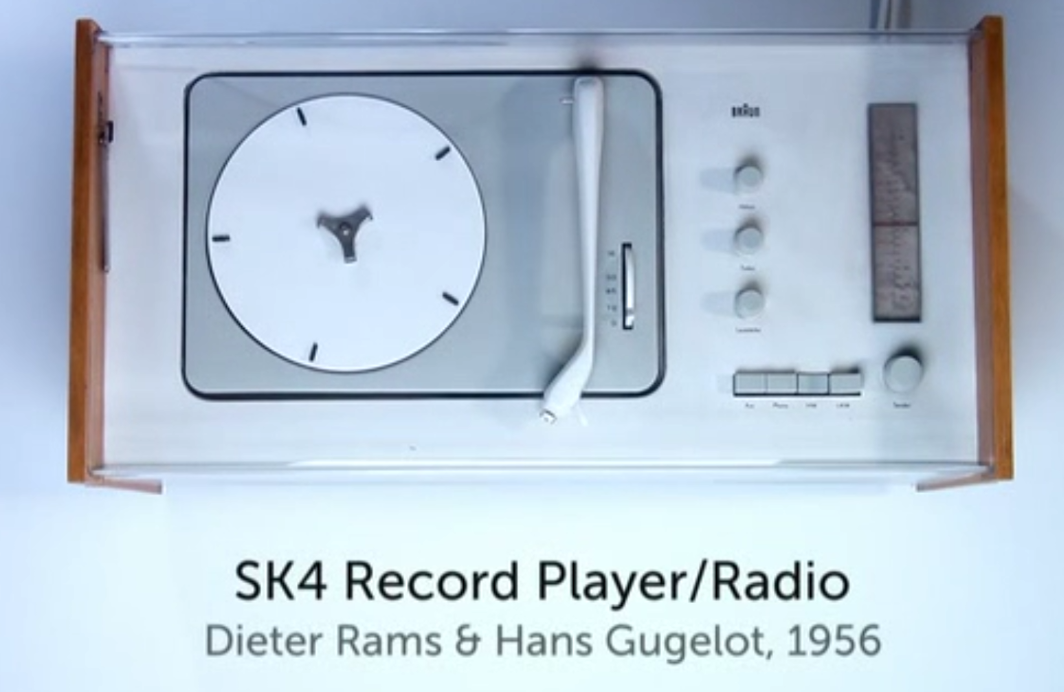
\includegraphics[width=0.5\textwidth]{./src/figures/Sk4 Record Player Radio_2023-04-09_20-40-36.png}
    \caption{[Dieter Rams and Hans Gugelot:Sk4 Record Player Radio]}
    \label{figure:Sk4 Record Player Radio}
\end{figure}


\begin{figure}[h]
    \centering
    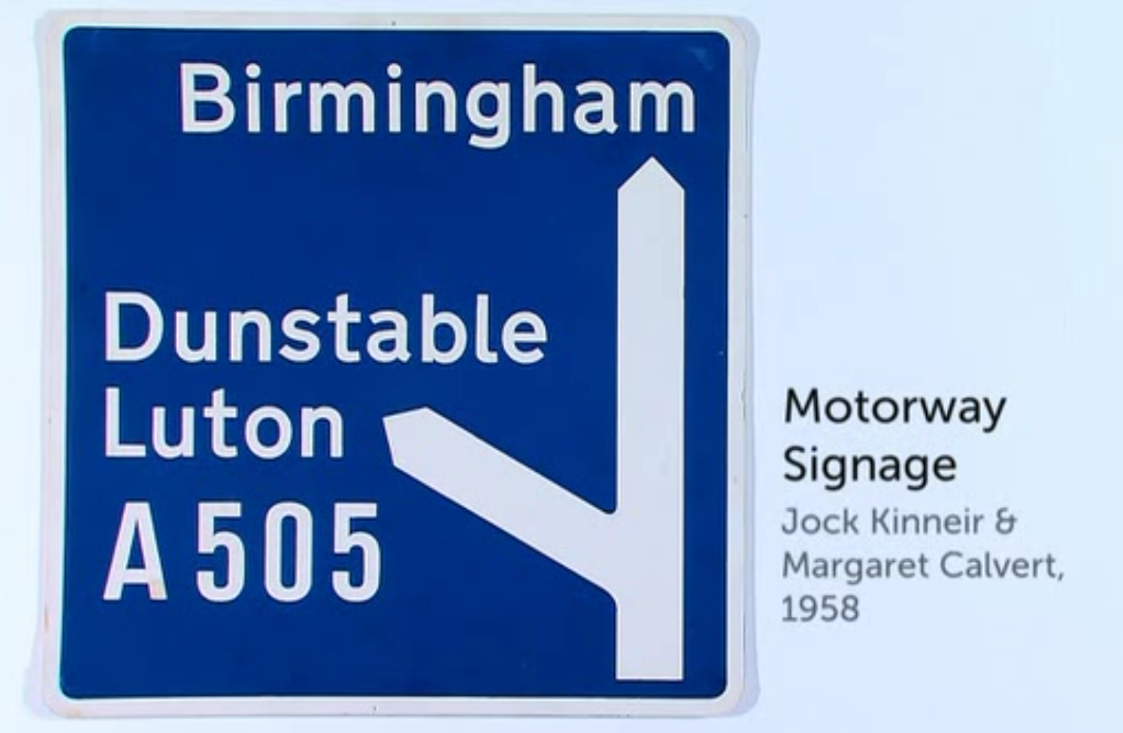
\includegraphics[width=0.5\textwidth]{./src/figures/Motorway Signage_2023-04-09_20-43-34.png}
    \caption{[Jock Kinneir and Margaret Calvert:Motorway Signage]}
    \label{figure:Motorway Signage}
\end{figure}




\begin{figure}[h]
    \centering
    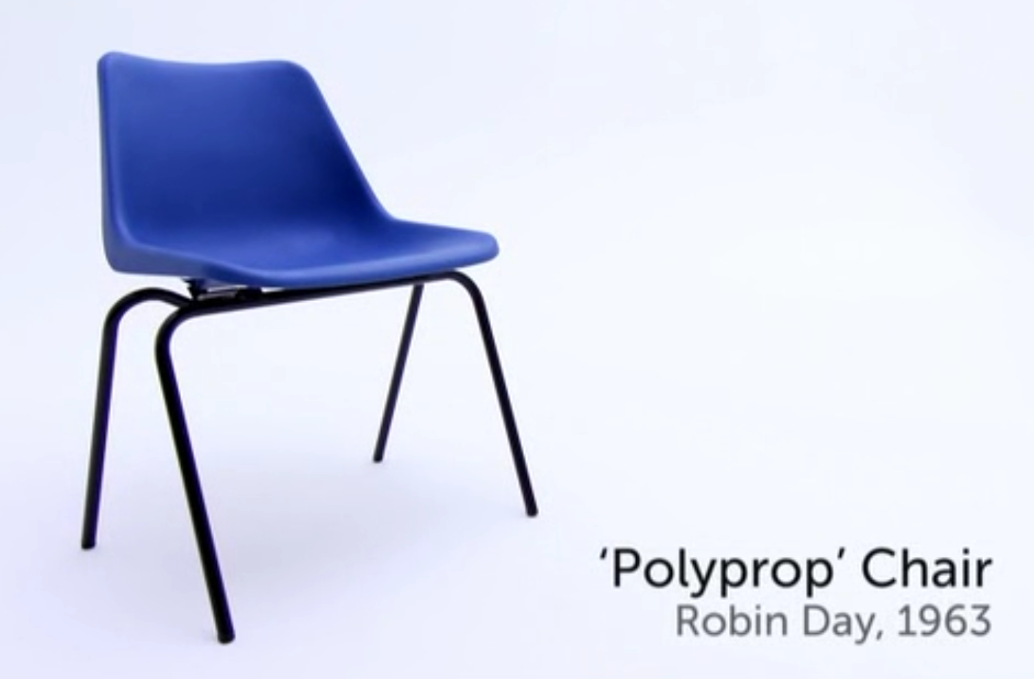
\includegraphics[width=0.5\textwidth]{./src/figures/Polyprop Chair_2023-04-09_20-46-07.png}
    \caption{[Robin Day:Polyprop Chair]}
    \label{figure:Polyprop Chair}
\end{figure}



\begin{figure}[h]
    \centering
    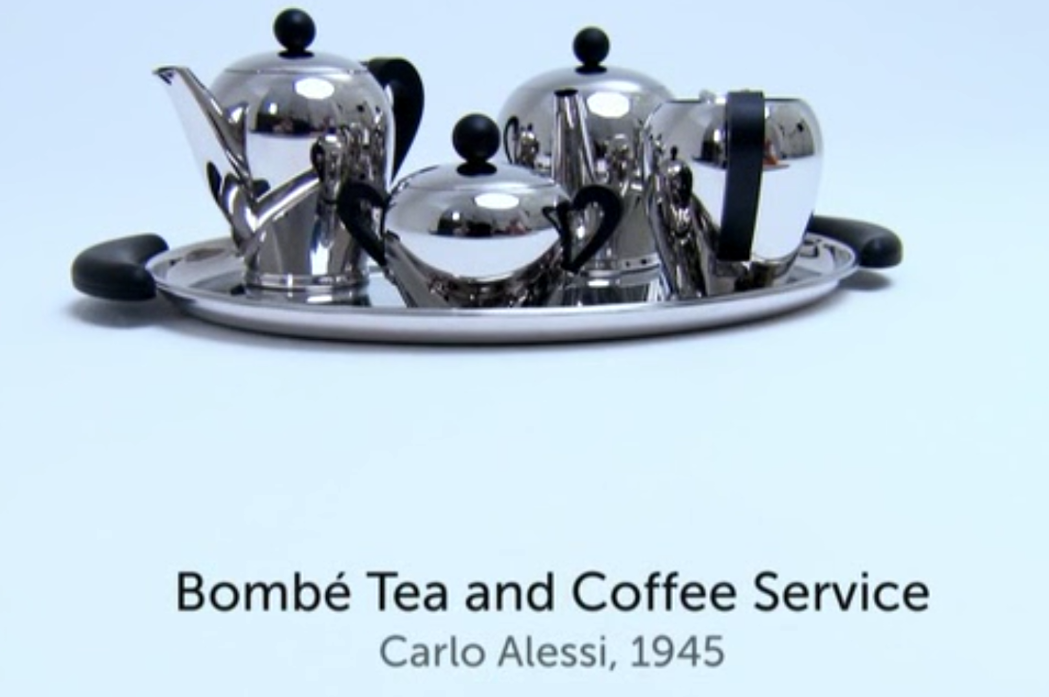
\includegraphics[width=0.5\textwidth]{./src/figures/Bombe Tea and Coffe Service_2023-04-09_20-49-08.png}
    \caption{[Carlo Alessi:Bombe Tea and Coffe Service]}
    \label{figure:Bombe Tea and Coffe Service}
\end{figure}

塑料不易长期保存,用后即丢的思想。转瞬即逝生活方式的象征。随意邂逅,不在乎人与人之间真正的关系。



\begin{figure}[h]
    \centering
    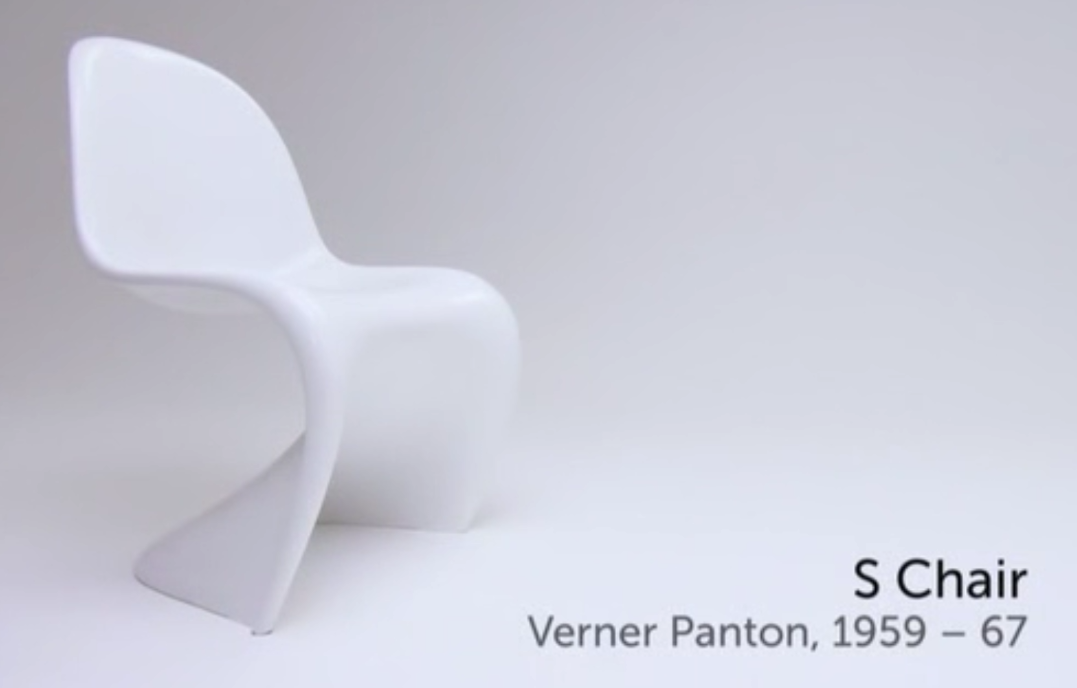
\includegraphics[width=0.5\textwidth]{./src/figures/S Chair_2023-04-09_20-54-06.png}
    \caption{[Verner Panton:S Chair]}
    \label{figure:S Chair}
\end{figure}


\begin{figure}[h]
    \centering
    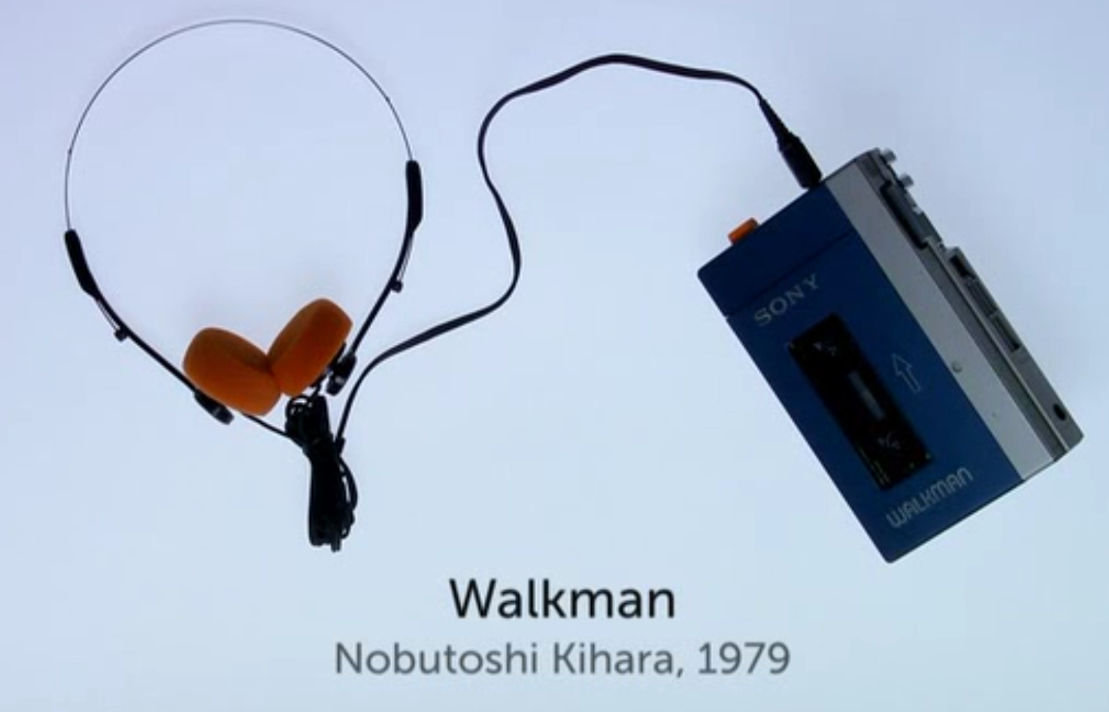
\includegraphics[width=0.5\textwidth]{./src/figures/Walkman_2023-04-09_20-59-42.png}
    \caption{[Nobutoshi Kihara:Walkman]}
    \label{figure:Walkman}
\end{figure}
索尼,小型化,新的生活方式。

一次性注塑的塑料椅。



【5】欲望之物

\begin{figure}[h]
    \centering
    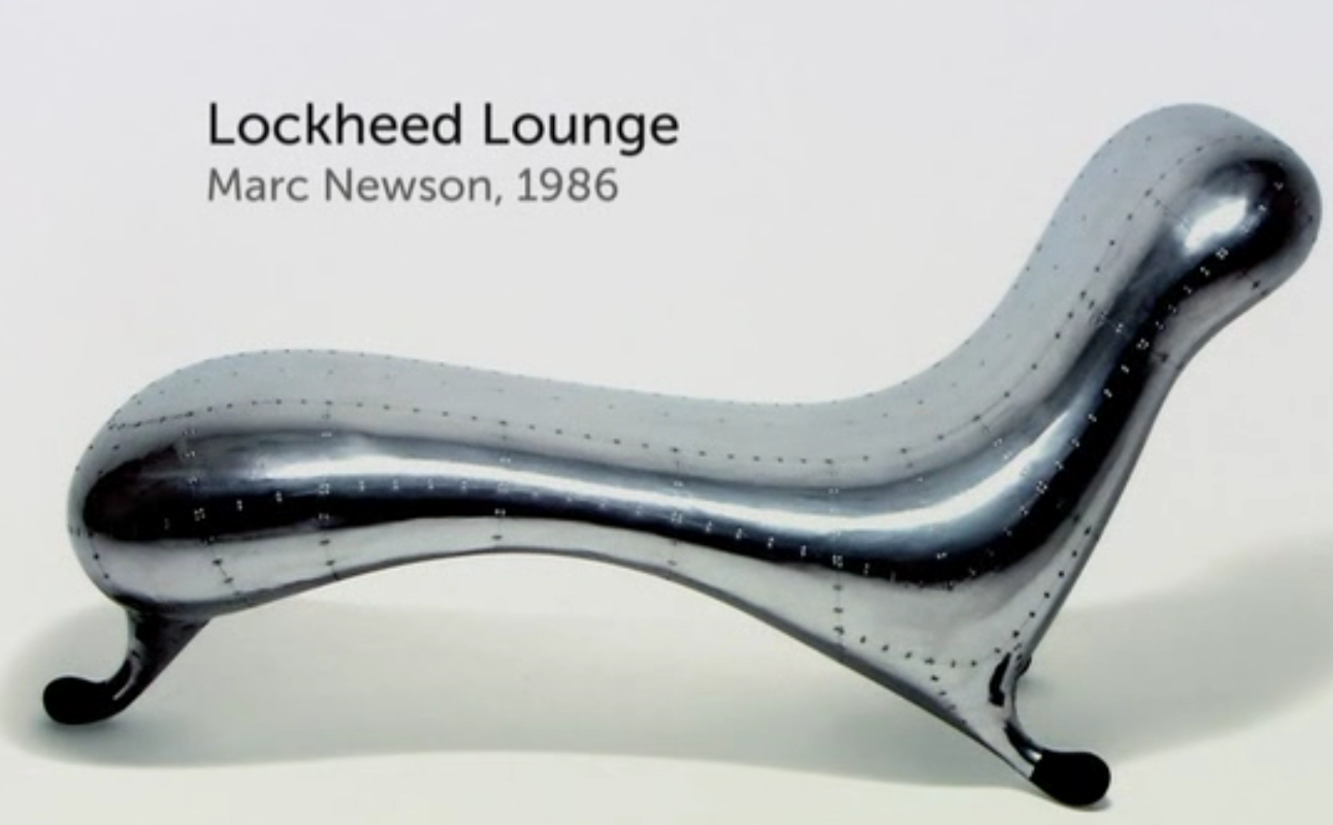
\includegraphics[width=0.5\textwidth]{./src/figures/Lockheed Lounge_2023-04-09_21-08-42.png}
    \caption{[Marc Newson:Lockheed Lounge]}
    \label{figure:Lockheed Lounge}
\end{figure}
拍卖2,434,500英镑。



\begin{figure}[h]
    \centering
    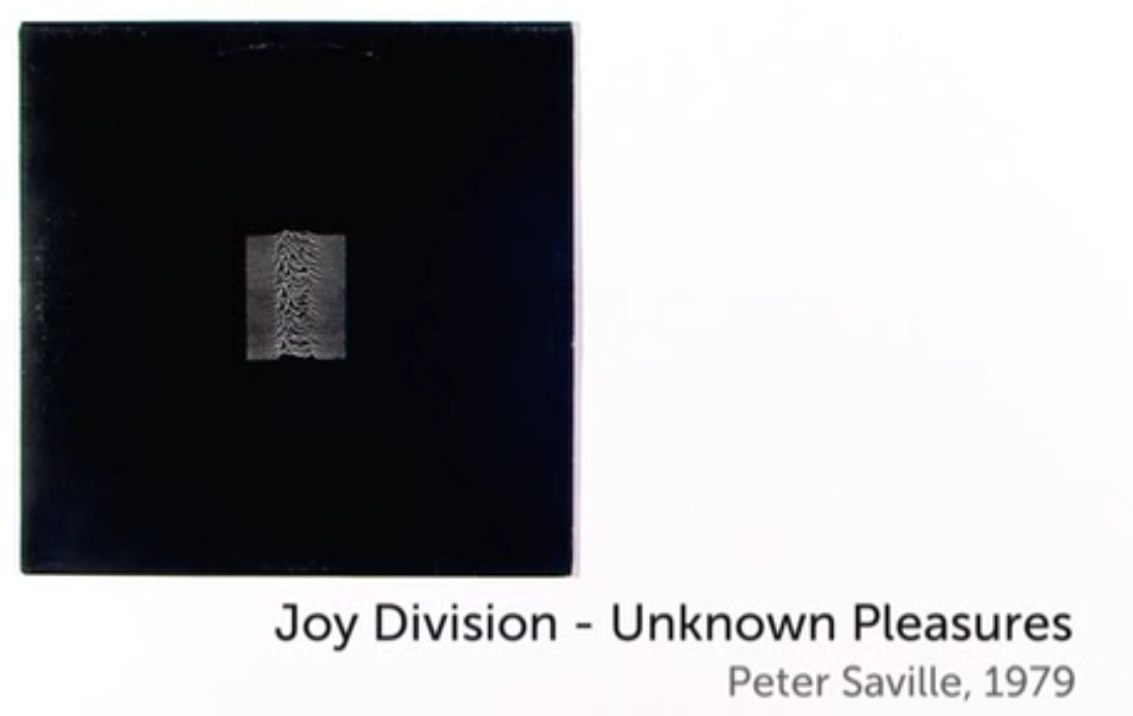
\includegraphics[width=0.5\textwidth]{./src/figures/Joy Division-Unknown Pleasures_2023-04-09_21-11-12.png}
    \caption{[Peter Saville:Joy Division-Unknown Pleasures]}
    \label{figure:Joy Division-Unknown Pleasures}
\end{figure}



\begin{figure}[h]
    \centering
    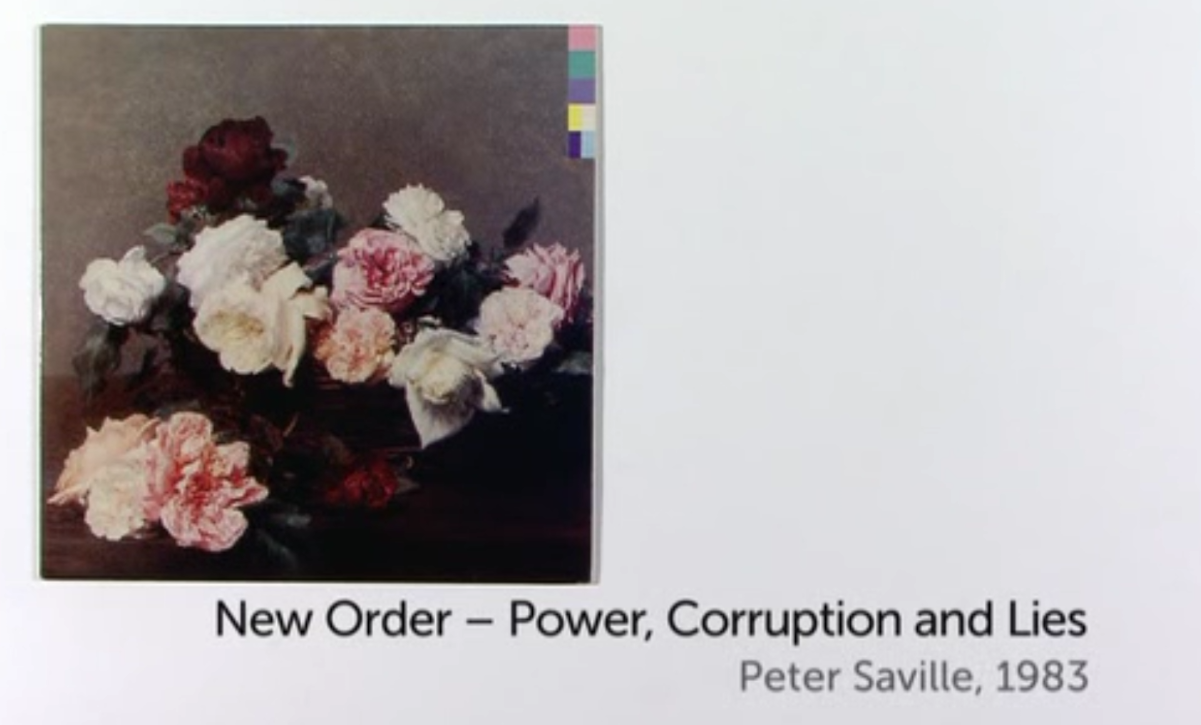
\includegraphics[width=0.5\textwidth]{./src/figures/New Order-Power, Corruption and Lies_2023-04-09_21-12-41.png}
    \caption{[Peter Saville:New Order-Power, Corruption and Lies]}
    \label{figure:New Order-Power, Corruption and Lies}
\end{figure}
直接用Fantin Latour的画作为自己的设计。表现的是人类深层次的占有欲。强化自我意识。



\begin{figure}[h]
    \centering
    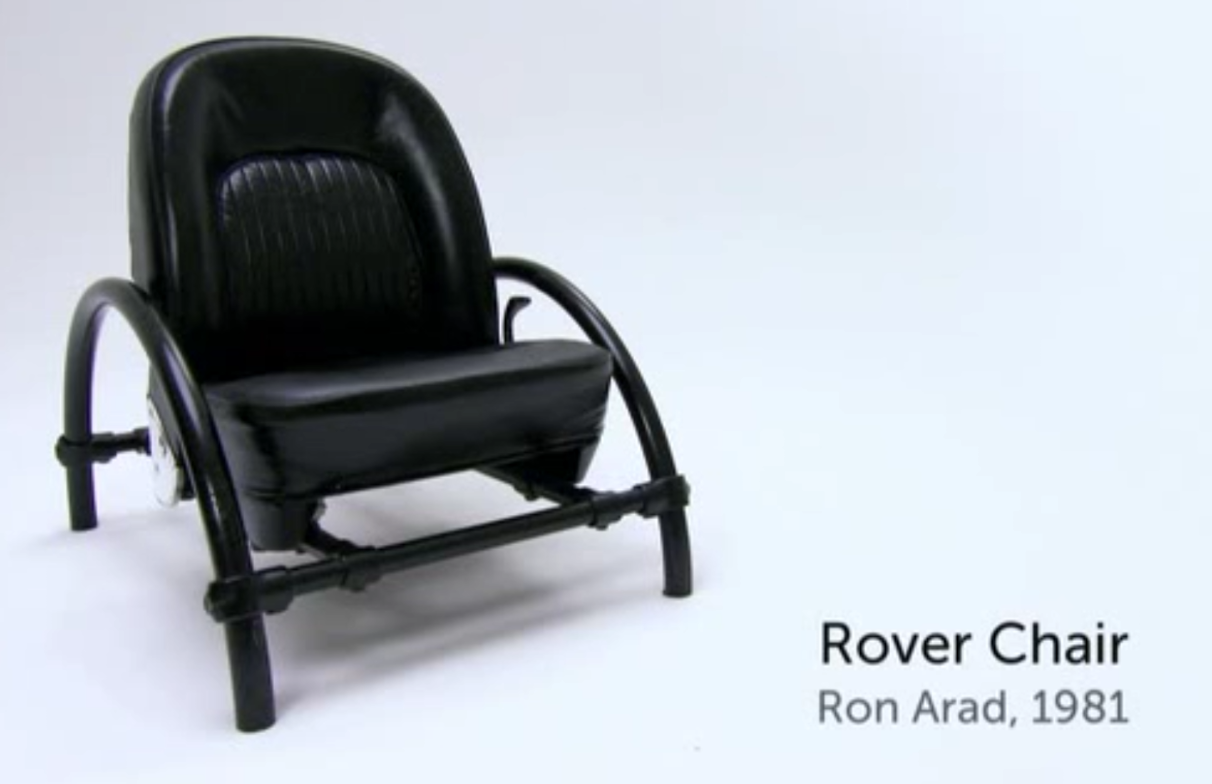
\includegraphics[width=0.5\textwidth]{./src/figures/Rover Chair_2023-04-09_21-16-06.png}
    \caption{[Ron Arad:Rover Chair]}
    \label{figure:Rover Chair}
\end{figure}
废品站的旧的汽车椅子,改成可调节椅背的椅子。




\begin{figure}[h]
    \centering
    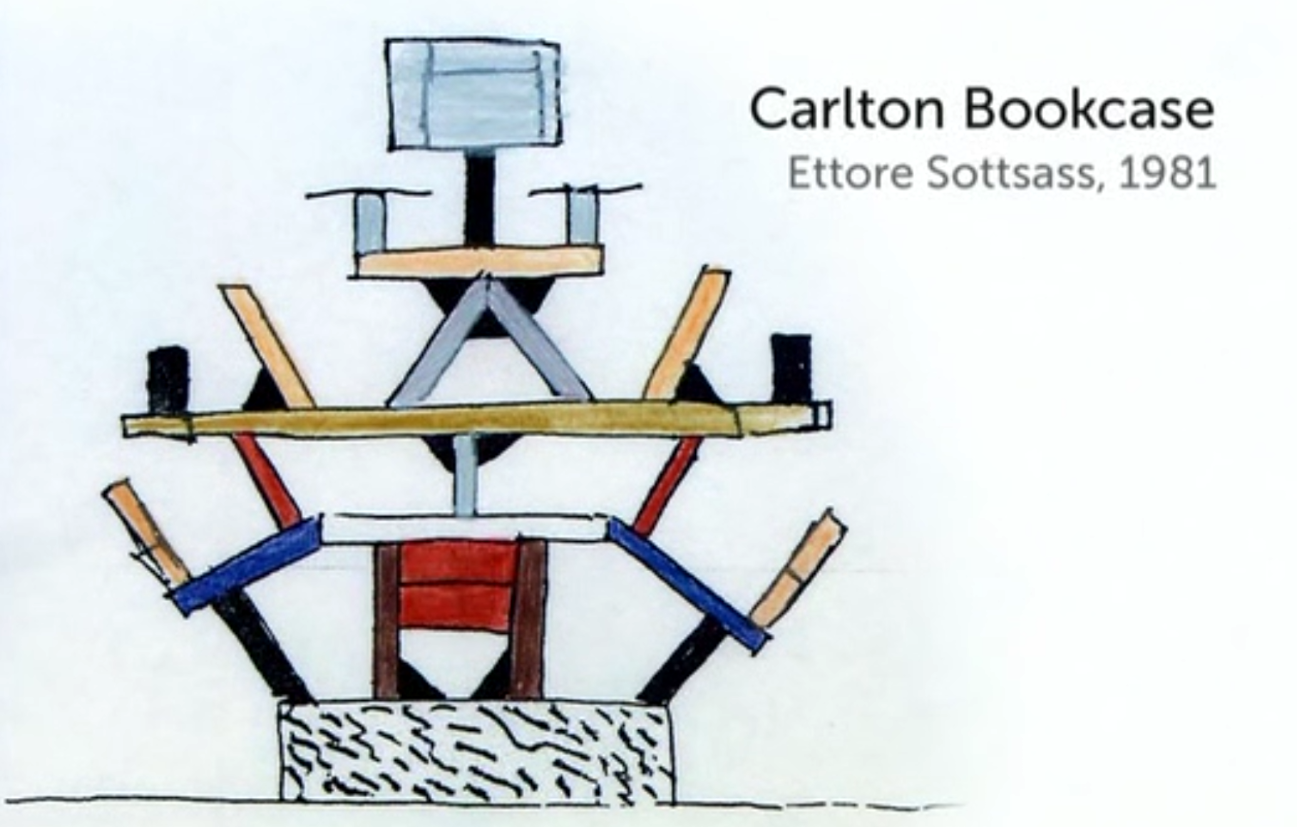
\includegraphics[width=0.5\textwidth]{./src/figures/Carlton Bookcase_2023-04-09_21-18-44.png}
    \caption{[Ettore Sottsass:Carlton Bookcase]}
    \label{figure:Carlton Bookcase}
\end{figure}


\begin{figure}[h]
    \centering
    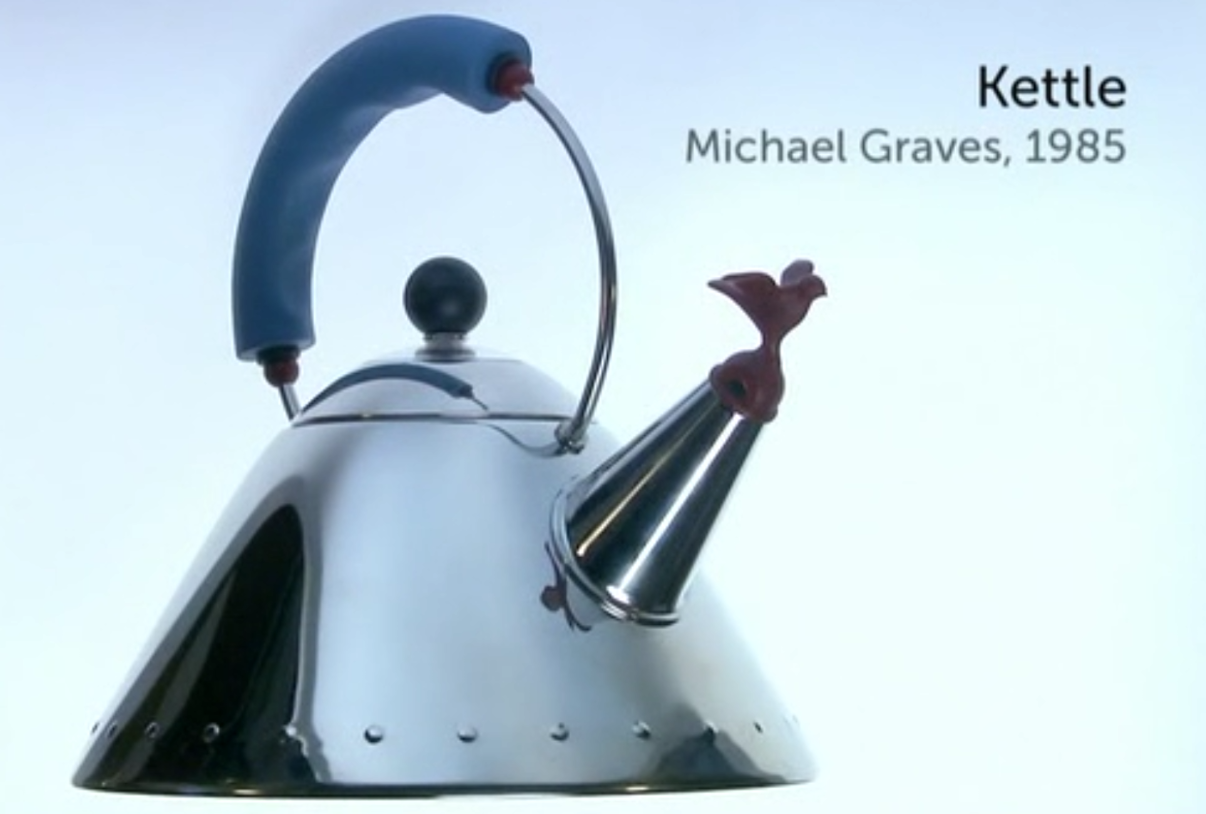
\includegraphics[width=0.5\textwidth]{./src/figures/Kettle_2023-04-09_21-21-57.png}
    \caption{[Michael Graves:Kettle]}
    \label{figure:Kettle}
\end{figure}

为什么感觉是虚伪的设计:要说明一项设计的成功、厉害,要么卖得贵,要么卖得数量多。



\begin{figure}[h]
    \centering
    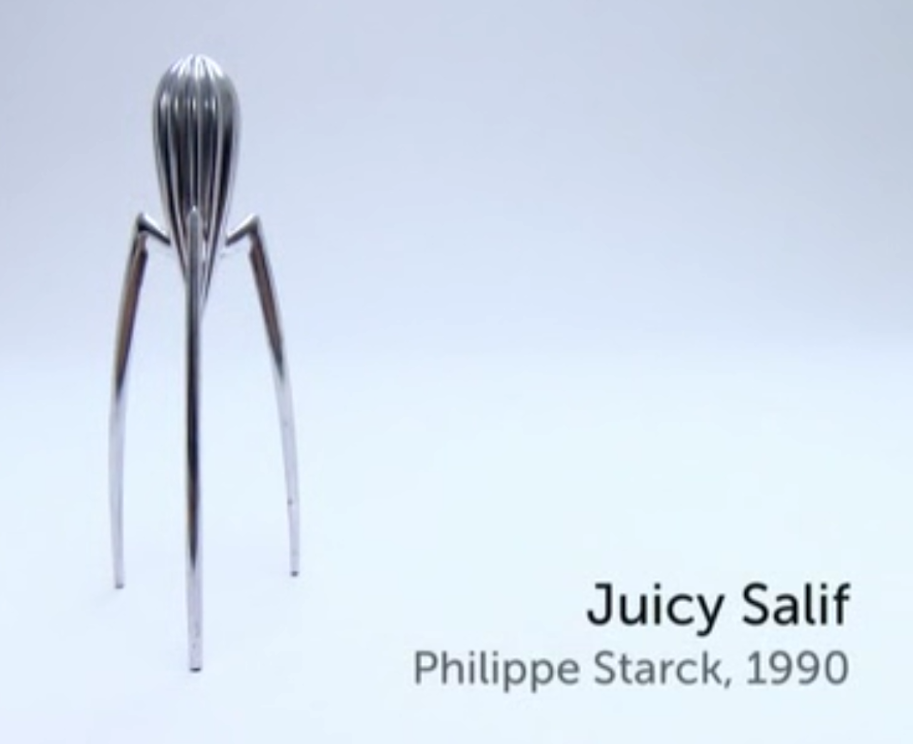
\includegraphics[width=0.5\textwidth]{./src/figures/Juicy Salif_2023-04-09_21-25-09.png}
    \caption{[Philippe Starck:Juicy Salif]}
    \label{figure:Juicy Salif}
\end{figure}


\begin{figure}[h]
    \centering
    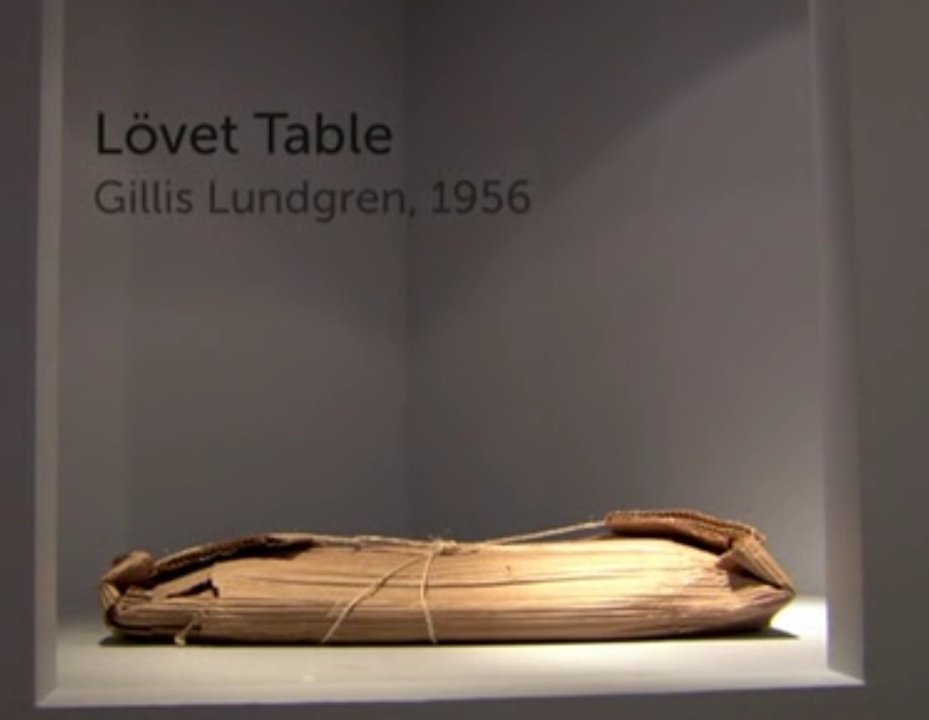
\includegraphics[width=0.5\textwidth]{./src/figures/Lovet Table_2023-04-09_21-30-09.png}
    \caption{[Gillis Lundgren:Lovet Table]}
    \label{figure:Lovet Table}
\end{figure}
宜家,桌子的3个腿可拆卸,方便运输、存放。


\begin{figure}[h]
    \centering
    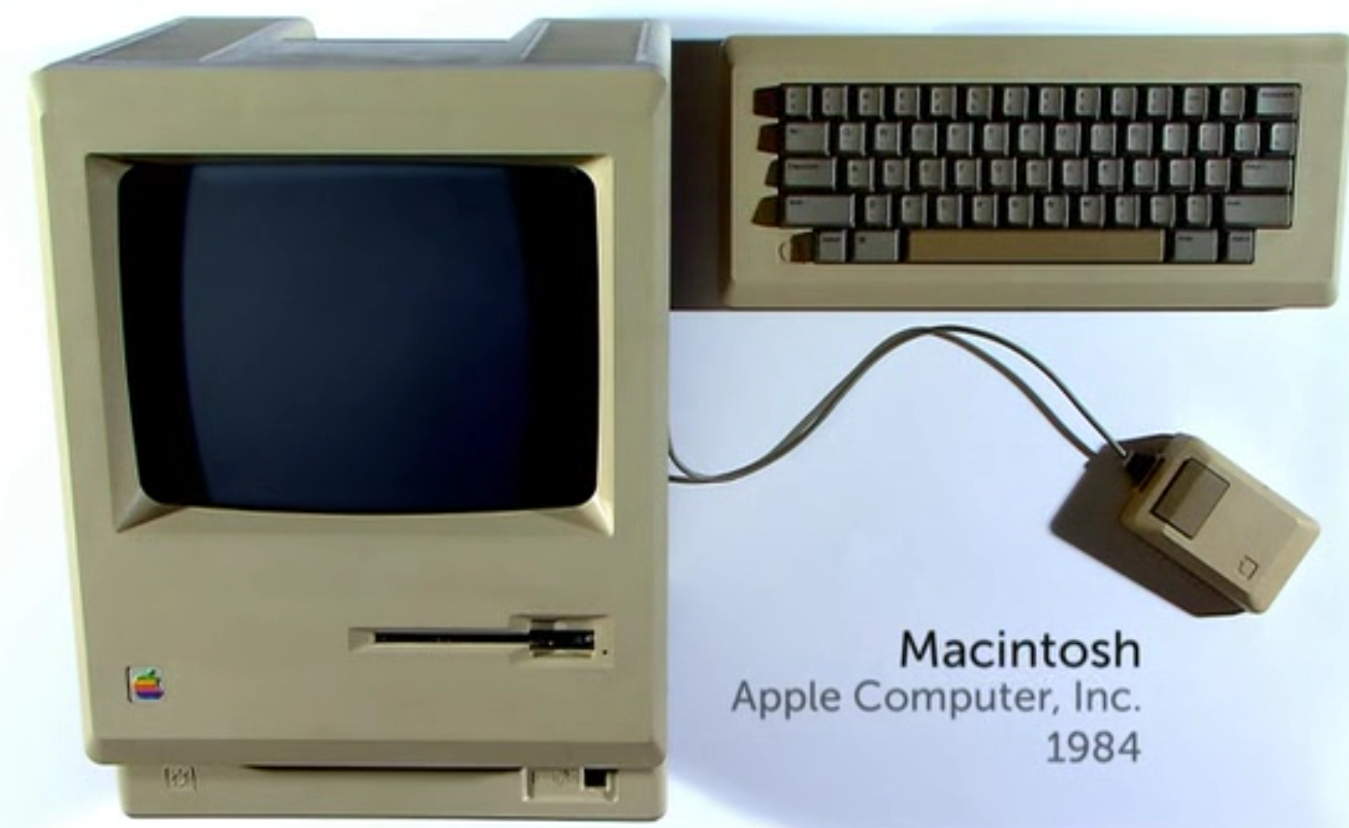
\includegraphics[width=0.5\textwidth]{./src/figures/Macintosh_2023-04-09_21-53-44.png}
    \caption{[Apple Computer:Macintosh]}
    \label{figure:Macintosh}
\end{figure}
苹果,personal computer


\begin{figure}[h]
    \centering
    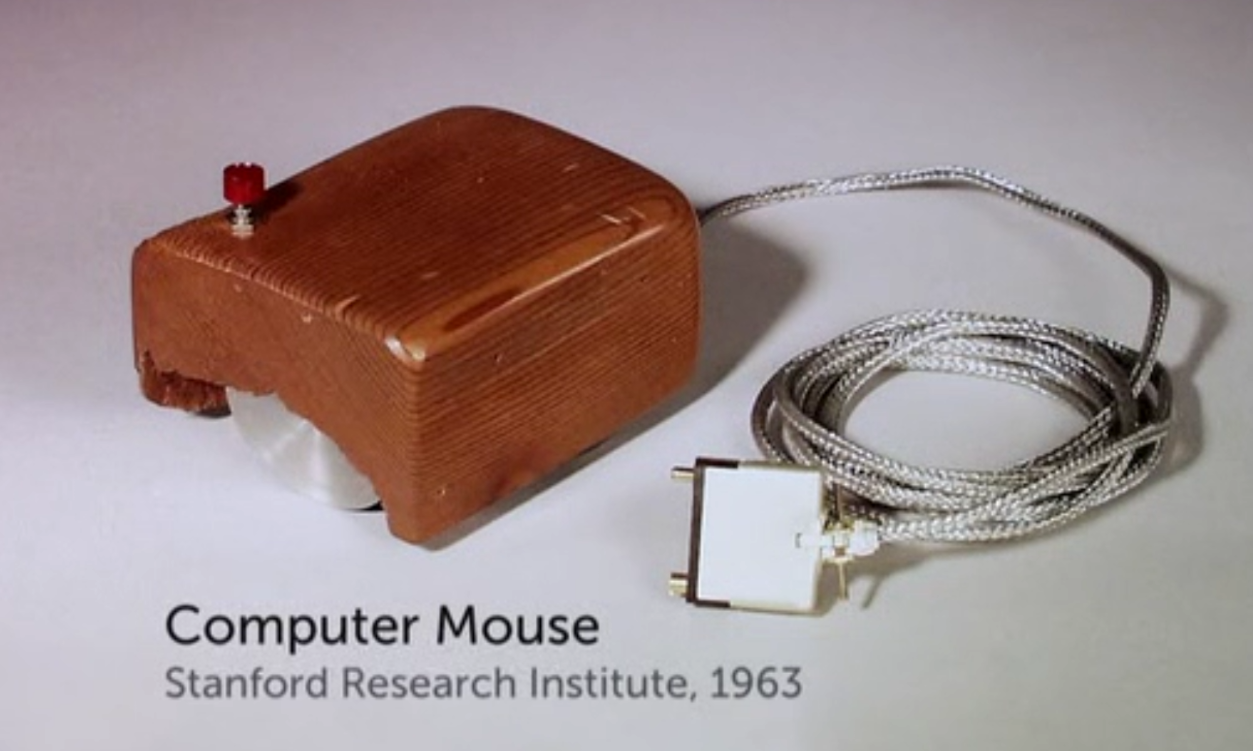
\includegraphics[width=0.5\textwidth]{./src/figures/Computer Mouse_2023-04-09_21-56-05.png}
    \caption{[Stanford Research Institute:Computer Mouse]}
    \label{figure:Computer Mouse}
\end{figure}


\begin{figure}[h]
    \centering
    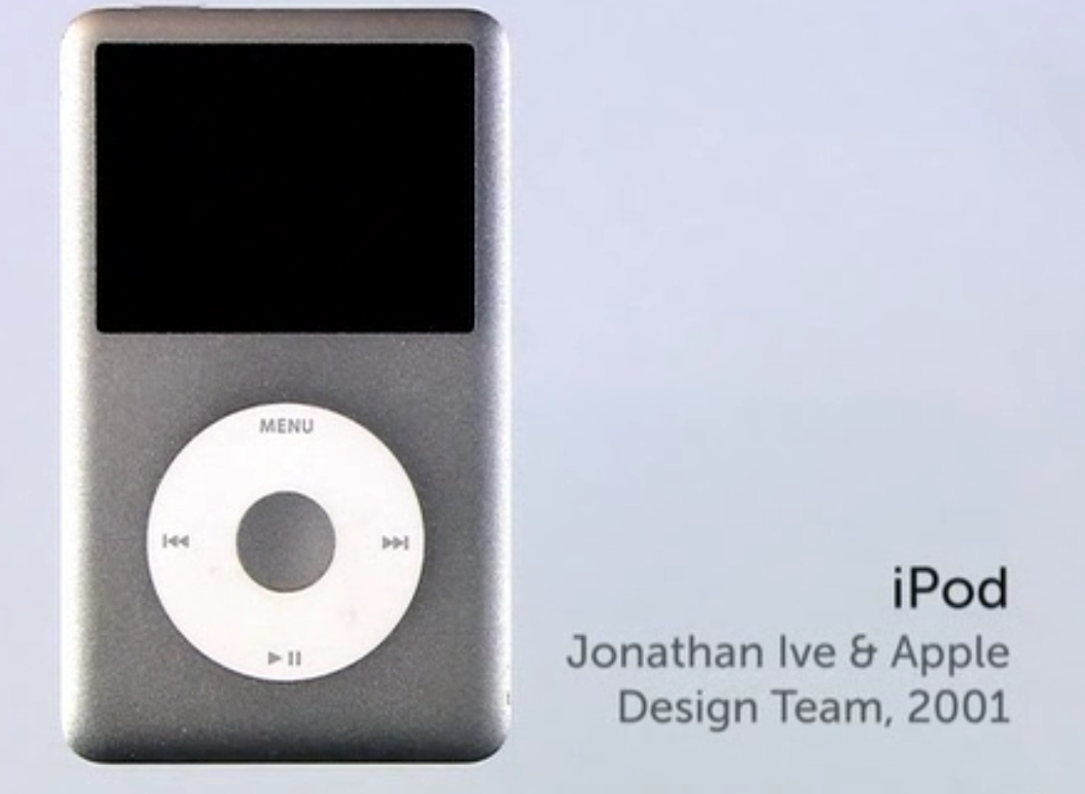
\includegraphics[width=0.5\textwidth]{./src/figures/iPod_2023-04-09_21-59-02.png}
    \caption{[Jonathan Ive and Apple Design Team:iPod]}
    \label{figure:iPod}
\end{figure}


\begin{figure}[h]
    \centering
    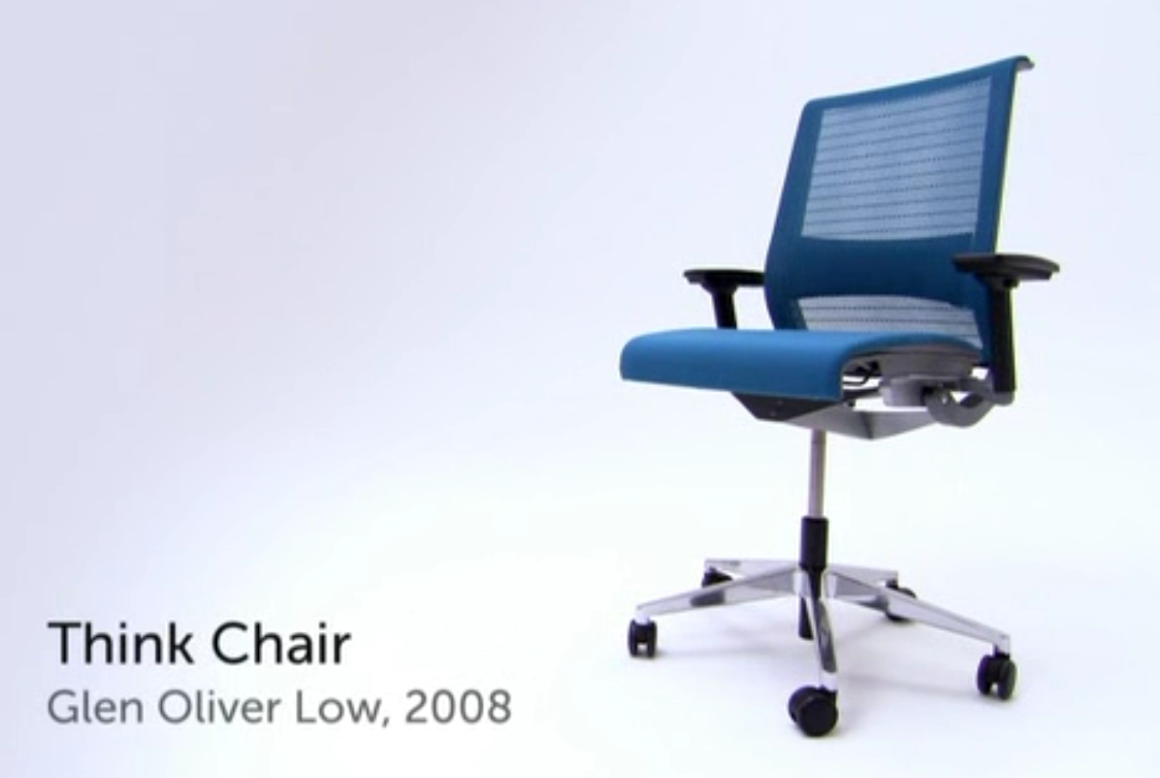
\includegraphics[width=0.5\textwidth]{./src/figures/Think Chair_2023-04-09_22-02-24.png}
    \caption{[Glean Oliver Low:Think Chair]}
    \label{figure:Think Chair}
\end{figure}
所有材料可以原模原样回收再利用的。无限回收再利用。


\end{document}

